\documentclass[conference]{IEEEtran}
\IEEEoverridecommandlockouts
% ---------------------------------------------------------------------------
% Beevil Knievel -- IEEE conference paper
% Every number in Section V can be regenerated with the scripts in analysis/
% (see README.md). Figures produced by the authors' repository are cited as such.
% ---------------------------------------------------------------------------
\usepackage[T1]{fontenc}
\usepackage{cite}
\usepackage{amsmath,amssymb,amsfonts}
\usepackage{graphicx}
\usepackage{textcomp}
\usepackage{xcolor}
\usepackage{booktabs}
\usepackage{multirow}
\usepackage{array}
\usepackage{siunitx}
\sisetup{per-mode=symbol, range-phrase= to , range-units=single}
\usepackage[caption=false,font=footnotesize]{subfig}
\usepackage{tikz}
\usetikzlibrary{arrows.meta,calc}
\usepackage{url}
\usepackage[hidelinks]{hyperref}

\newcommand{\evT}{\textsf{T}}  % tested
\newcommand{\evA}{\textsf{A}}  % analysed
\newcommand{\evS}{\textsf{S}}  % simulated
\newcommand{\evP}{\textsf{P}}  % planned
\newcommand{\evD}{\textsf{D}}  % demonstrated (UI)
\newcommand{\COtwo}{CO\textsubscript{2}}
\raggedbottom

\begin{document}

\title{Beevil Knievel: An Edge-Native LoRa Cyber-Physical System for Non-Invasive In-Comb Honeybee Colony Health Monitoring}

\author{\IEEEauthorblockN{Atharve Dahima}
\IEEEauthorblockA{\textit{Department of Electronics and Communication Engineering}\\
\textit{Malaviya National Institute of Technology Jaipur}\\
Jaipur, India\\
atharvedahima@gmail.com}
\and
\IEEEauthorblockN{Srajan Mishra}
\IEEEauthorblockA{\textit{Department of Electronics and Communication Engineering}\\
\textit{Malaviya National Institute of Technology Jaipur}\\
Jaipur, India\\
srajanmishra@gmail.com}
\and
\IEEEauthorblockN{Vishal Sharma}
\IEEEauthorblockA{\textit{Department of Electronics and Communication Engineering}\\
\textit{Malaviya National Institute of Technology Jaipur}\\
Jaipur, India\\
vishal.ece@mnit.ac.in}
}

\maketitle

\begin{abstract}
Routine honeybee colony inspection is invasive, labour-intensive and leaves multi-week blind spots in which queen loss, brood chilling or swarming go unnoticed. This paper presents Beevil Knievel, an open, edge-native cyber-physical system in which a Nordic nRF52840/Semtech SX1262 node instruments a Langstroth hive with brood-core, frame, acoustic, \COtwo, gas, mass, tilt and light sensing, compresses each observation into a 33-byte binary frame with explicit not-connected sentinels, and forwards it over IN865 LoRa to a hardened Raspberry Pi gateway that persists, diagnoses and streams colony state to offline operator interfaces. Because the prototype is at bench level, we separate tested, analysed and simulated evidence and report only results that can be regenerated from the public repository. All 29 automated tests pass, and the gateway sustains 265 to 336 frames/s over five runs (99th-percentile latency below \SI{8.1}{ms}), roughly 800 times the load of a 100-hive apiary. Datasheet- and model-based analyses show that the frame needs \SI{71.9}{ms} of airtime at SF7, that uncoordinated access limits one channel to 21 hives at 99\% delivery, that ground-level links span \SIrange{0.6}{2.7}{km} rather than tens of kilometres, and that NDIR \COtwo{} sensing consumes 85\% of node energy; duty-cycling it extends 2600-mAh autonomy from 181 to 545 days. Monte-Carlo analysis shows that the firmware brood-cooling CUSUM false-alarms within hours under autocorrelated variability, whereas a re-tuned Page CUSUM reaches a 34-day in-control run length with sub-hour detection of a \SI{1}{\celsius} drop. We further expose a cross-tier alert-encoding defect, quantify the gain sensitivity of the acoustic decision engine, and report first-pass ANSYS thermal, structural, modal and electromagnetic models together with their limitations.
\end{abstract}

\begin{IEEEkeywords}
Precision apiculture, cyber-physical systems, LoRa, edge computing, change-point detection, bioacoustics, energy budgeting, Internet of Things.
\end{IEEEkeywords}

% ===========================================================================
\section{Introduction}
% ===========================================================================
Honeybees (\textit{Apis mellifera}) supply a large share of the animal pollination on which crop production depends: the value of insect pollination was estimated at \texteuro153 billion per year~\cite{gallai2009}, and pollinator declines are driven by interacting pressures from land use, pesticides, pathogens and climate~\cite{potts2010}. Managed colonies remain fragile. A coordinated U.S. survey estimated a 55.6\% loss of managed colonies between April 2024 and April 2025, the highest on record~\cite{auburn2025}, and 39.9\% in the following year~\cite{auburn2026}.

Most beekeepers still assess colony health by opening the hive every one to three weeks (Fig.~\ref{fig:context}). Each inspection breaks the propolis seal, releases nest heat and disturbs the colony, while the conditions that matter most (brood chilling after queen failure, the build-up to swarming, and winter starvation) develop unobserved between visits. Precision beekeeping addresses this gap with continuous sensing of hive temperature, weight and sound~\cite{zacepins2015,meikle2015}. Wireless prototypes have demonstrated in-hive thermal-pattern detection~\cite{kridi2016}, decision-tree health analysis~\cite{edwardsmurphy2016} and multi-sensor monitoring~\cite{cecchi2020}, and bio-acoustic and vibrational studies have linked spectral changes to swarming~\cite{ferrari2008,bencsik2011,ramsey2020} and to queenlessness~\cite{nolasco2018,ruvinga2023}.

Turning these findings into deployable systems requires solving several coupled problems at once: sensing inside the brood nest without disturbing it, extracting decision-relevant features on a microcontroller, delivering them over kilometre-scale links on a battery budget, and operating a gateway that survives rural power cuts without cloud connectivity. Prototype reports also often blur the boundary between measured, simulated and aspirational performance, which makes them hard to reproduce or compare.

This paper presents \emph{Beevil Knievel}~\cite{beevilrepo}, an open-source three-tier system that targets these problems, and evaluates it with an explicit separation of evidence classes. Source code and simulation models are openly available on GitHub (\url{https://github.com/atharveeee-netizen/beevil-knievel}). Our contributions are:
\begin{enumerate}
\item an edge-native architecture and a compact, sentinel-aware 33-byte telemetry contract that links an nRF52840/SX1262 field node to a Raspberry Pi gateway with offline persistence, rule-based diagnosis and live operator interfaces (Section~\ref{sec:arch});
\item a reproducible software validation: 29 automated tests, an independent ingestion benchmark and a cross-tier encoding test that uncovers an alert-flag collision (Sections~\ref{sec:m-sw} and~\ref{sec:r-sw});
\item datasheet- and model-grounded analyses of LoRa airtime, medium-access scaling and ground-level range, and a bottom-up node energy budget that identifies \COtwo{} sensing as the dominant load (Sections~\ref{sec:r-radio} and~\ref{sec:r-energy});
\item a Monte-Carlo characterisation and re-tuning of the brood-cooling CUSUM detector, and robustness audits of the acoustic decision engine and of the gateway classifier (Sections~\ref{sec:r-cusum}--\ref{sec:r-rf});
\item a transparent account of first-pass multiphysics models and of the remaining gap to field validation (Sections~\ref{sec:r-sim} and~\ref{sec:disc}).
\end{enumerate}
Section~\ref{sec:related} reviews related work, Section~\ref{sec:arch} describes the architecture, Section~\ref{sec:methods} the evaluation methods and Section~\ref{sec:results} the results; Section~\ref{sec:disc} discusses limitations and Section~\ref{sec:concl} concludes.

\begin{figure}[!t]
\centering
\subfloat[]{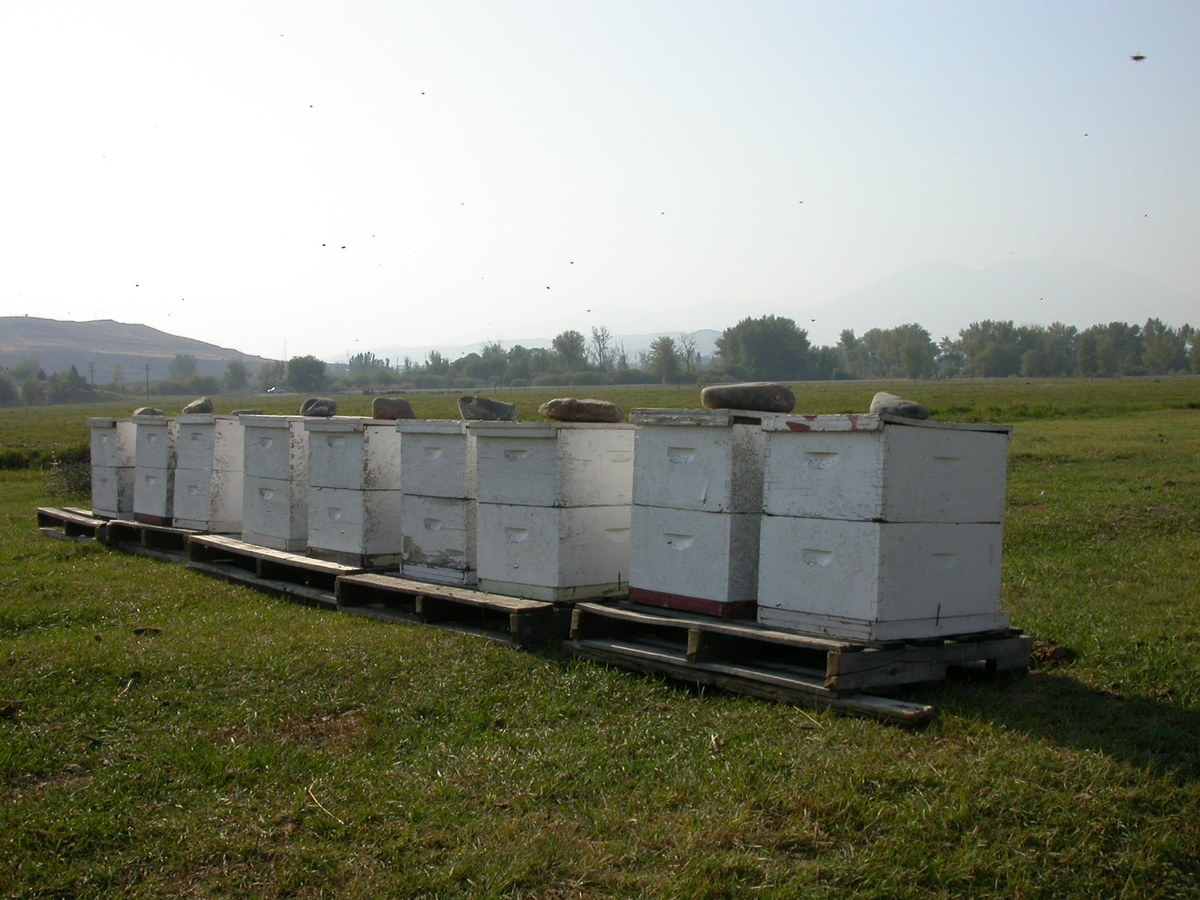
\includegraphics[height=3.05cm]{figs/photo_usda_apiary.jpg}\label{fig:ctx-a}}\hfil
\subfloat[]{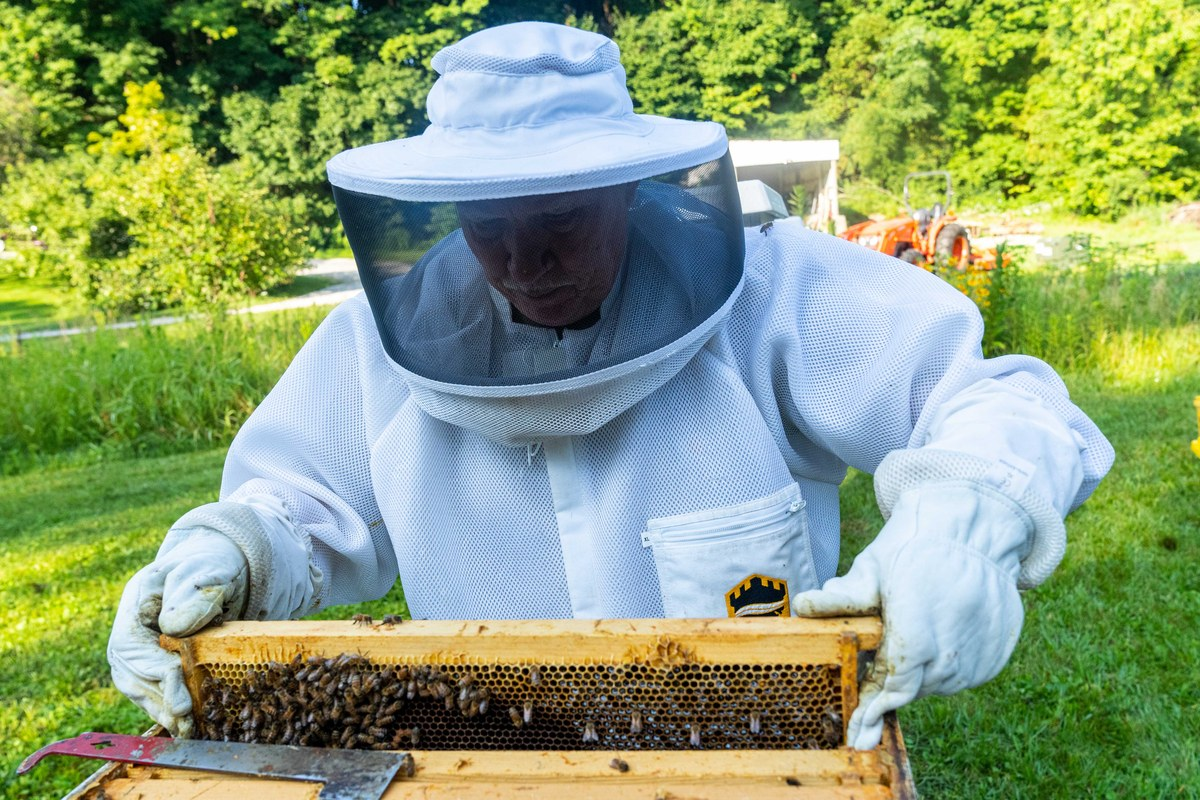
\includegraphics[height=3.05cm]{figs/photo_usda_inspection.jpg}\label{fig:ctx-b}}
\caption{Operational context. (a) A commercial Langstroth apiary and (b) a manual frame inspection, the status-quo method that opens the brood nest. Photographs: U.S. Department of Agriculture (public domain).}
\label{fig:context}
\end{figure}

% ===========================================================================
\section{Related Work}\label{sec:related}
% ===========================================================================
\textit{Continuous hive monitoring.} Healthy colonies regulate brood temperature within roughly \SIrange{34.5}{35.5}{\celsius} through metabolic heating and fanning~\cite{southwick1987,seeley1985}, so a sustained drift of the brood-nest temperature is an early sign of failing thermoregulation. Kridi \textit{et al.}~\cite{kridi2016} detected in-hive thermal patterns with a wireless sensor network; Edwards-Murphy \textit{et al.}~\cite{edwardsmurphy2016} combined heterogeneous sensors with decision-tree analysis; Cecchi \textit{et al.}~\cite{cecchi2020} built a multi-sensor measurement system including audio; Meikle and Holst~\cite{meikle2015} reviewed continuous weight and temperature monitoring, and Zacepins \textit{et al.}~\cite{zacepins2015} identified power autonomy and data interpretation as open challenges. Our design follows these lines but places the temperature reference inside the comb, adds \COtwo{} and gas sensing, and performs feature extraction on the node so that a low-rate radio suffices.

\textit{Acoustic and vibrational indicators.} Ferrari \textit{et al.}~\cite{ferrari2008} observed changes in hive sound frequency together with temperature before swarming; Bencsik \textit{et al.}~\cite{bencsik2011} and Ramsey \textit{et al.}~\cite{ramsey2020} identified and predicted swarming from vibrational spectra. Nolasco and Benetos released annotated recordings from the Open Source Beehive and NU-Hive projects~\cite{nolasco2018,nolasco2018data}, later used for queen-presence detection~\cite{ruvinga2023}, and Zgank~\cite{zgank2020} classified swarm activity for an IoT farm service. These studies analyse recordings offline or on gateway-class hardware; we ask which spectral summaries survive on a microcontroller and inside a 33-byte radio frame.

\textit{LPWAN scaling and change detection.} LoRa trades data rate for sensitivity~\cite{augustin2016,semtech2013an}, and its capacity is limited by airtime and collisions under ALOHA-like access~\cite{abramson1970,bor2016,adelantado2017}. Page's CUSUM~\cite{page1954,montgomery2013} suits the slow thermal drifts that precede brood loss, but its false-alarm rate depends strongly on the in-control variability and autocorrelation, which we quantify explicitly.

% ===========================================================================
\section{System Architecture}\label{sec:arch}
% ===========================================================================
Fig.~\ref{fig:arch} summarises the three tiers. Table~\ref{tab:frame} lists the field-node sensors together with the telemetry fields they populate, and Table~\ref{tab:status} states the implementation status and evidence class of every subsystem.

\begin{figure*}[!t]
\centering
\resizebox{\textwidth}{!}{%
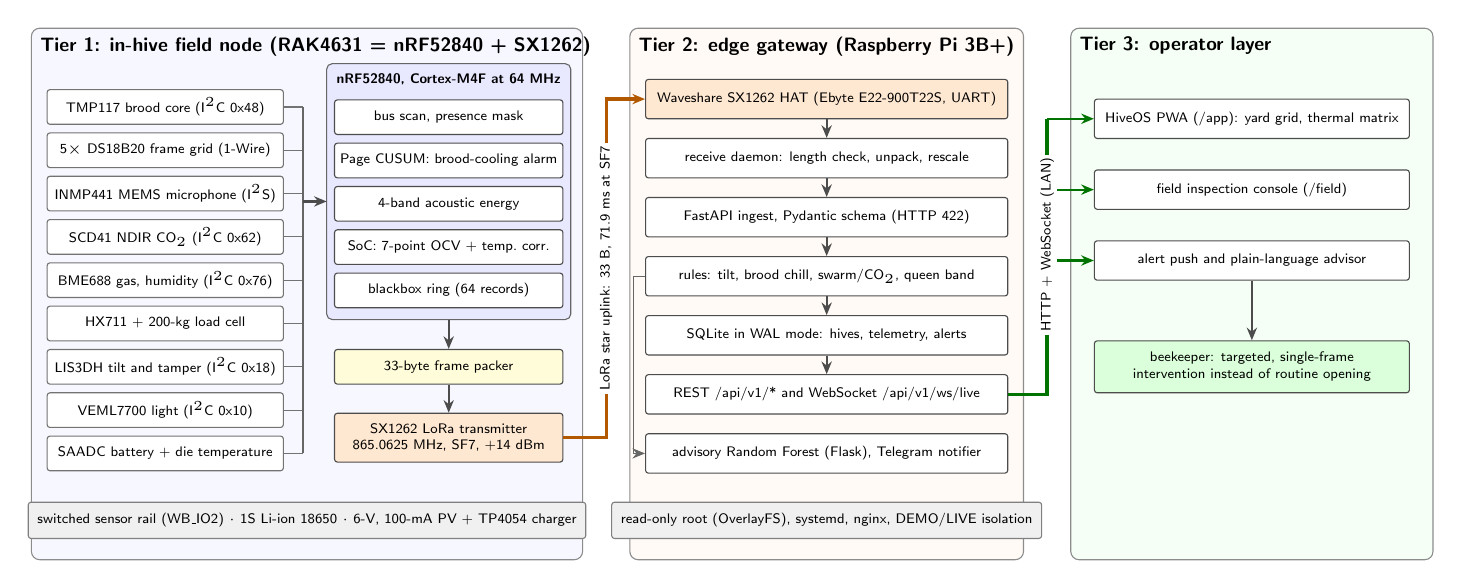
\begin{tikzpicture}[font=\sffamily\scriptsize, >={Stealth[length=1.6mm,width=1.3mm]},
 sens/.style={draw=black!55, fill=white, rounded corners=1pt, minimum width=3.0cm, minimum height=0.44cm, inner sep=1pt, align=center, font=\sffamily\tiny},
 proc/.style={draw=black!70, fill=white, rounded corners=1pt, minimum width=2.9cm, minimum height=0.44cm, inner sep=1pt, align=center, font=\sffamily\tiny},
 gw/.style={draw=black!70, fill=white, rounded corners=1pt, minimum width=4.6cm, minimum height=0.5cm, inner sep=1pt, align=center, font=\sffamily\tiny},
 ui/.style={draw=black!70, fill=white, rounded corners=1pt, minimum width=4.0cm, minimum height=0.5cm, inner sep=1pt, align=center, font=\sffamily\tiny},
 hdr/.style={font=\sffamily\scriptsize\bfseries, anchor=north west, inner sep=3pt},
 lnk/.style={font=\sffamily\tiny, fill=white, inner sep=1pt, rotate=90}]
% tier backgrounds
\filldraw[draw=black!45, fill=blue!3, rounded corners=3pt] (0,0) rectangle (7.0,6.75);
\filldraw[draw=black!45, fill=orange!4, rounded corners=3pt] (7.6,0) rectangle (12.6,6.75);
\filldraw[draw=black!45, fill=green!4, rounded corners=3pt] (13.2,0) rectangle (17.8,6.75);
\node[hdr] at (0,6.75) {Tier 1: in-hive field node (RAK4631 = nRF52840 + SX1262)};
\node[hdr] at (7.6,6.75) {Tier 2: edge gateway (Raspberry Pi 3B+)};
\node[hdr] at (13.2,6.75) {Tier 3: operator layer};
% tier 1: sensors
\node[sens] at (1.7,5.75) {TMP117 brood core (I$^2$C 0x48)};
\node[sens] at (1.7,5.20) {5$\times$ DS18B20 frame grid (1-Wire)};
\node[sens] at (1.7,4.65) {INMP441 MEMS microphone (I$^2$S)};
\node[sens] at (1.7,4.10) {SCD41 NDIR CO$_2$ (I$^2$C 0x62)};
\node[sens] at (1.7,3.55) {BME688 gas, humidity (I$^2$C 0x76)};
\node[sens] at (1.7,3.00) {HX711 + 200-kg load cell};
\node[sens] at (1.7,2.45) {LIS3DH tilt and tamper (I$^2$C 0x18)};
\node[sens] at (1.7,1.90) {VEML7700 light (I$^2$C 0x10)};
\node[sens] at (1.7,1.35) {SAADC battery + die temperature};
\foreach \y in {5.75,5.20,4.65,4.10,3.55,3.00,2.45,1.90,1.35} {\draw[black!55] (3.2,\y) -- (3.45,\y);}
\draw[black!60, line width=0.9pt] (3.45,1.35) -- (3.45,5.75);
% tier 1: MCU block
\filldraw[draw=black!60, fill=blue!9, rounded corners=2pt] (3.75,3.05) rectangle (6.85,6.3);
\node[font=\sffamily\tiny\bfseries, anchor=north] at (5.3,6.3) {nRF52840, Cortex-M4F at 64 MHz};
\draw[->, thick, black!70] (3.45,4.55) -- (3.75,4.55);
\node[proc] (p1) at (5.3,5.62) {bus scan, presence mask};
\node[proc] (p2) at (5.3,5.07) {Page CUSUM: brood-cooling alarm};
\node[proc] (p3) at (5.3,4.52) {4-band acoustic energy};
\node[proc] (p4) at (5.3,3.97) {SoC: 7-point OCV + temp.\ corr.};
\node[proc] (p5) at (5.3,3.42) {blackbox ring (64 records)};
\node[proc, fill=yellow!15] (pk) at (5.3,2.45) {33-byte frame packer};
\node[proc, fill=orange!18, minimum height=0.62cm] (tx) at (5.3,1.55) {SX1262 LoRa transmitter\\865.0625 MHz, SF7, +14 dBm};
\draw[->, thick, black!70] (5.3,3.05) -- (pk.north);
\draw[->, thick, black!70] (pk.south) -- (tx.north);
\node[draw=black!50, fill=black!6, rounded corners=1pt, minimum width=6.6cm, minimum height=0.46cm, font=\sffamily\tiny, align=center] at (3.5,0.5) {switched sensor rail (WB\_IO2) $\cdot$ 1S Li-ion 18650 $\cdot$ 6-V, 100-mA PV + TP4054 charger};
% tier 2
\node[gw, fill=orange!18] (g1) at (10.1,5.85) {Waveshare SX1262 HAT (Ebyte E22-900T22S, UART)};
\node[gw] (g2) at (10.1,5.10) {receive daemon: length check, unpack, rescale};
\node[gw] (g3) at (10.1,4.35) {FastAPI ingest, Pydantic schema (HTTP 422)};
\node[gw] (g4) at (10.1,3.60) {rules: tilt, brood chill, swarm/CO$_2$, queen band};
\node[gw] (g5) at (10.1,2.85) {SQLite in WAL mode: hives, telemetry, alerts};
\node[gw] (g6) at (10.1,2.10) {REST /api/v1/* and WebSocket /api/v1/ws/live};
\node[gw] (g7) at (10.1,1.35) {advisory Random Forest (Flask), Telegram notifier};
\node[draw=black!50, fill=black!6, rounded corners=1pt, minimum width=4.6cm, minimum height=0.46cm, font=\sffamily\tiny, align=center] at (10.1,0.5) {read-only root (OverlayFS), systemd, nginx, DEMO/LIVE isolation};
\foreach \a/\b in {g1/g2,g2/g3,g3/g4,g4/g5,g5/g6} {\draw[->, thick, black!70] (\a.south) -- (\b.north);}
\draw[->, black!60] (g4.west) -- ++(-0.15,0) |- (g7.west);
% tier 3 (Playdate emulator removed)
\node[ui] (u1) at (15.5,5.60) {HiveOS PWA (/app): yard grid, thermal matrix};
\node[ui] (u2) at (15.5,4.70) {field inspection console (/field)};
\node[ui] (u4) at (15.5,3.80) {alert push and plain-language advisor};
\node[ui, fill=green!14, minimum height=0.66cm] (u5) at (15.5,2.45) {beekeeper: targeted, single-frame\\intervention instead of routine opening};
\draw[->, thick, black!70] (u4.south) -- (u5.north);
% links
\draw[->, very thick, orange!70!black] (tx.east) -- (7.3,1.55) -- (7.3,5.85) -- (g1.west);
\node[lnk] at (7.3,3.7) {LoRa star uplink: 33 B, 71.9 ms at SF7};
\draw[very thick, green!45!black] (g6.east) -- (12.9,2.10) -- (12.9,5.60);
\foreach \u in {u1,u2,u4} {\draw[->, thick, green!45!black] (12.9,0|-\u.west) -- (\u.west);}
\node[lnk] at (12.9,4.0) {HTTP + WebSocket (LAN)};
\end{tikzpicture}}
\caption{Beevil Knievel architecture. Tier~1 converts in-hive physical quantities into a 33-byte frame on the node; Tier~2 validates, diagnoses, stores and publishes it on a power-loss-hardened gateway without cloud dependency; Tier~3 presents colony state and alerts to the beekeeper.}
\label{fig:arch}
\end{figure*}

\subsection{Tier 1: In-Hive Field Node}\label{sec:node}
The node is built on a RAKwireless RAK4631 WisBlock core, which integrates a Nordic nRF52840 (Arm Cortex-M4F at \SI{64}{MHz}, \SI{1}{MB} flash, \SI{256}{KB} RAM)~\cite{nrf52840ps} and a Semtech SX1262 sub-GHz transceiver~\cite{sx1262ds,rak4631ds}, mounted on a RAK5005-O base board. The sensors of Table~\ref{tab:frame} share a \SI{400}{kHz} I$^2$C bus, a 1-Wire bus for five DS18B20 frame probes and an I$^2$S bus for the INMP441 microphone, and are supplied from a rail switched by a GPIO (WB\_IO2) so that they draw no current while the node sleeps. A 1S Li-ion cell (18650, \SIrange{2.6}{3.0}{Ah}) charged by the base board's linear charger (\SI{4.20}{V} termination) from a \SI{6}{V}, \SI{100}{mA} panel powers the node.

The firmware (PlatformIO, \texttt{nordicnrf52} 11.0.0, Arduino framework) follows a \emph{never-fabricate} rule. At boot it scans its buses and builds an 8-bit presence mask; a sensor that does not acknowledge is serialised as a sentinel ($-9999$ for signed temperatures, \texttt{0xFFFF} for unsigned 16-bit fields, \texttt{0xFF} for tilt) rather than a placeholder value. The on-node algorithms are (i) a brood-cooling CUSUM detector (Section~\ref{sec:m-cusum}); (ii) a state-of-charge estimator that interpolates a seven-point open-circuit-voltage table between \SI{3.27}{V} (0\%) and \SI{4.20}{V} (100\%) after a linear temperature correction of the 12-bit SAADC reading; (iii) a 64-record blackbox ring that keeps \SI{5.3}{h} of history at \SI{5}{min} intervals across gateway outages; and (iv) the acoustic band-energy front end (Section~\ref{sec:m-acoustic}). A serial console (\texttt{SCAN}, \texttt{SOC}, \texttt{CUSUM}, \texttt{BLACKBOX}, \texttt{TELEMETRY}) emits JSON-lines records tagged with their provenance. The authors' build of the bench firmware uses \SI{10.6}{kB} of RAM (4.3\%) and \SI{65.3}{kB} of flash (8.0\%); the committed v1.0.0 transmitter image occupies \SI{53.8}{kB} above the S140 SoftDevice.

\begin{table}[!t]
\caption{Field-Node Sensors and the 33-Byte Telemetry Frame}
\label{tab:frame}
\centering
\resizebox{\columnwidth}{!}{%
\begin{tabular}{@{}llllc@{}}
\toprule
Bytes & Field (type, scale) & Source (interface) & Range & Sentinel\\
\midrule
0--1   & hive ID (u16)                    & ---                         & 1--65535                     & ---\\
2--3   & brood core temp.\ (i16, $\times$100) & TMP117 (I$^2$C), $\pm$\SI{0.1}{\celsius} & \SIrange{-40}{85}{\celsius} & $-9999$\\
4--13  & frame temp.\ $\times$5 (i16, $\times$100) & DS18B20 (1-Wire), $\pm$\SI{0.5}{\celsius} & \SIrange{-40}{85}{\celsius} & $-9999$\\
14--15 & rel.\ humidity (u16, $\times$100) & BME688 (I$^2$C)           & 0--100\%                      & \texttt{FFFF}\\
16--17 & gas resistance (u16, $\times$10) & BME688 (I$^2$C)             & \SIrange{0}{6553.5}{\kilo\ohm} & \texttt{FFFF}\\
18--19 & \COtwo{} (u16)                   & SCD41 (I$^2$C)              & \SIrange{400}{5000}{ppm}      & \texttt{FFFF}\\
20--21 & hive mass (u16, $\times$100)     & HX711 + load cell           & \SIrange{0}{200}{kg}          & \texttt{FFFF}\\
22--23 & illuminance (u16)                & VEML7700 (I$^2$C)           & \SIrange{0}{65535}{lx}        & \texttt{FFFF}\\
24     & tilt (u8)$^{\dagger}$            & LIS3DH (I$^2$C)             & \SIrange{0}{90}{\degree}      & \texttt{FF}\\
25--32 & band energy $\times$8 (u8)       & INMP441 (I$^2$S)            & 0--255                        & 0\\
\bottomrule
\end{tabular}}
\\[2pt]\parbox{\columnwidth}{\footnotesize $^{\dagger}$The firmware also ORs alert flags into this byte; see Section~\ref{sec:r-sw}. Struct format \texttt{<Hh5hHHHHHB8B} (little-endian).}
\end{table}

\subsection{Telemetry Contract}\label{sec:contract}
Each observation is packed into the little-endian structure of Table~\ref{tab:frame}. Physical quantities use fixed-point scaling, and eight normalised acoustic band energies occupy one byte each. Compared with the compact JSON encoding used on the gateway API (251 bytes for the same content), the binary frame is 7.6 times smaller and needs 5.5 times less airtime at SF7 (\SI{71.9}{ms} versus \SI{394.5}{ms}). An optional 8-byte mesh header (source, destination, sequence number, hop count, time-to-live) extends the frame to 41 bytes (\SI{87.3}{ms}) for multi-hop relaying with duplicate suppression; the gateway side of this protocol is implemented and tested, while the deployed topology is a single-hop star.

\subsection{Tier 2: Edge Gateway}\label{sec:gateway}
The gateway (Fig.~\ref{fig:gateway}) is a Raspberry Pi 3B+ (BCM2837B0, four Cortex-A53 cores at \SI{1.4}{GHz}, \SI{1}{GB} RAM) with a Waveshare SX1262 LoRa HAT. A receive daemon checks the frame length, unpacks and rescales the fields and posts them to a local FastAPI service. The service validates them against a Pydantic schema (out-of-range values are rejected with HTTP 422), applies the diagnostic engine, stores the result in SQLite in write-ahead-logging (WAL) mode, including tables \texttt{hives}, \texttt{telemetry} and \texttt{alerts} with composite time indices, and pushes it to subscribers over a WebSocket. The diagnostic engine is an ordered rule set: tilt above \SI{15}{\degree} indicates tamper or theft; a brood core below \SI{31.5}{\celsius} indicates thermal stress; swarm-band energy above 0.65 or \COtwo{} above \SI{2800}{ppm} indicates a pre-swarm state; and queen-band energy below 0.18 indicates queenless distress. Its decision score grows with the margin by which a rule is exceeded. A separate advisory service hosts a Random-Forest model (Section~\ref{sec:m-rf}). Deployment scripts configure a read-only root file system with a RAM overlay (OverlayFS) so that the SD card survives abrupt power loss, together with systemd units, an nginx reverse proxy, a CORS allow-list and strict separation between a DEMO mode, which seeds 100 synthetic hives, and a LIVE mode, which starts empty. A Telegram notifier and a rule-augmented text advisor turn unresolved alerts into plain-language messages.

\begin{figure}[!t]
\centering
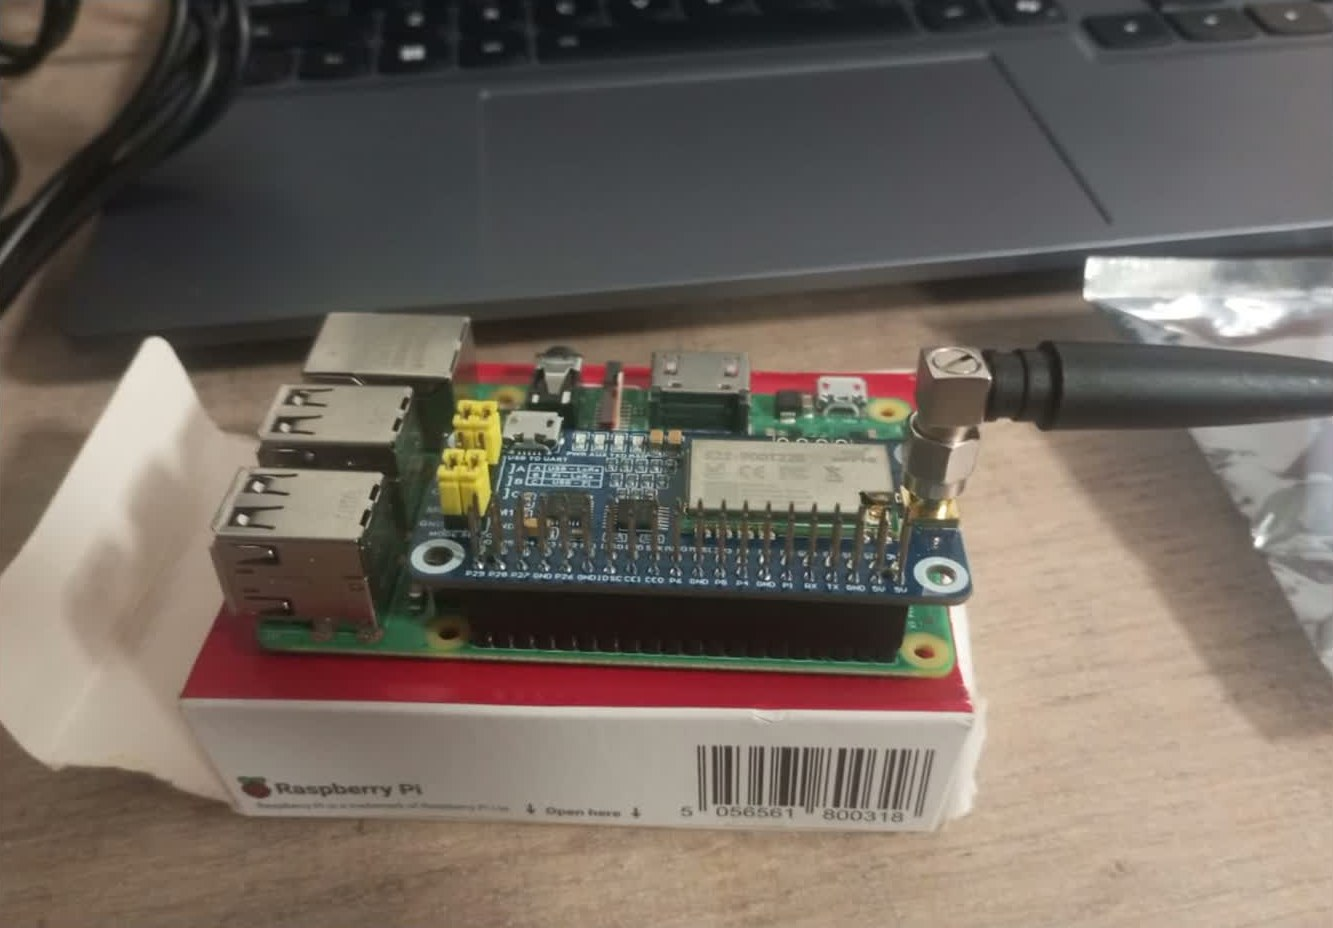
\includegraphics[width=0.86\columnwidth]{figs/photo_gateway.jpg}
\caption{Gateway prototype: Raspberry Pi 3B+ with a Waveshare SX1262 HAT built around an Ebyte E22-900T22S module and an \SI{865}{MHz} antenna (photograph from the project repository).}
\label{fig:gateway}
\end{figure}

\subsection{Tier 3: Operator Interfaces}
A Next.js progressive web application provides an apiary overview, a per-hive view with the five-frame thermal matrix and acoustic summary, and a field-inspection console (Fig.~\ref{fig:ui}). All screens in Fig.~\ref{fig:ui} were captured in DEMO mode and show synthetic data.

\begin{figure*}[!t]
\centering
\subfloat[]{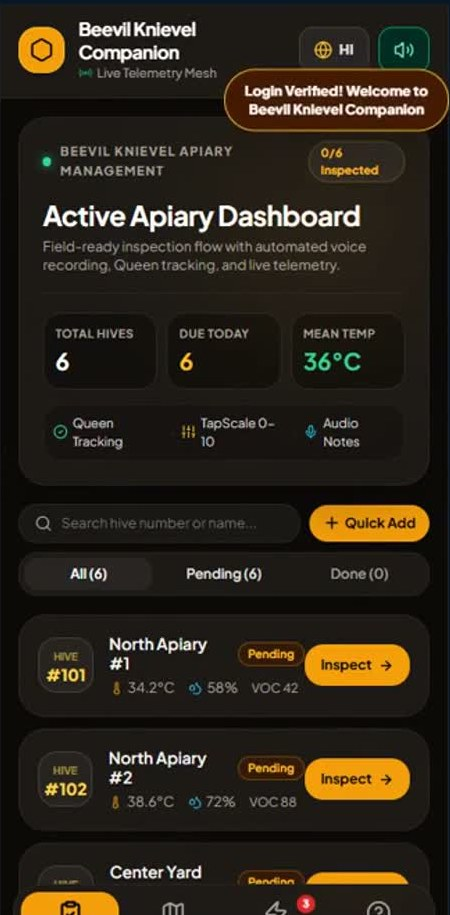
\includegraphics[width=0.31\textwidth]{figs/ui_companion.jpg}}\hfil
\subfloat[]{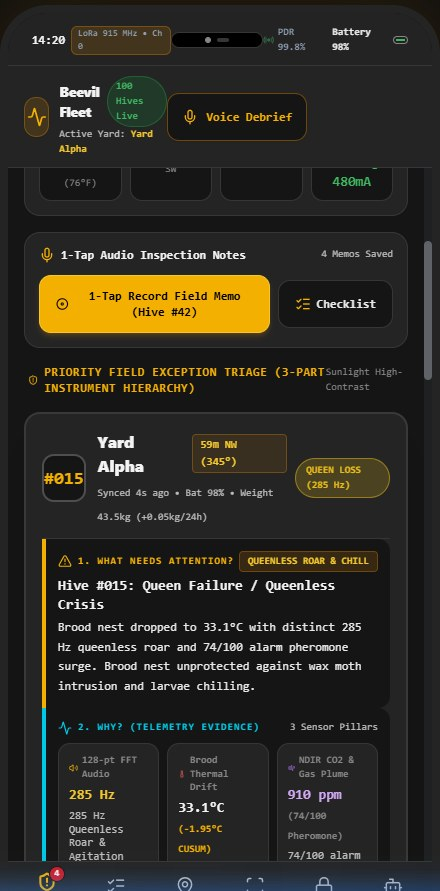
\includegraphics[width=0.31\textwidth]{figs/ui_hive_detail.jpg}}\hfil
\subfloat[]{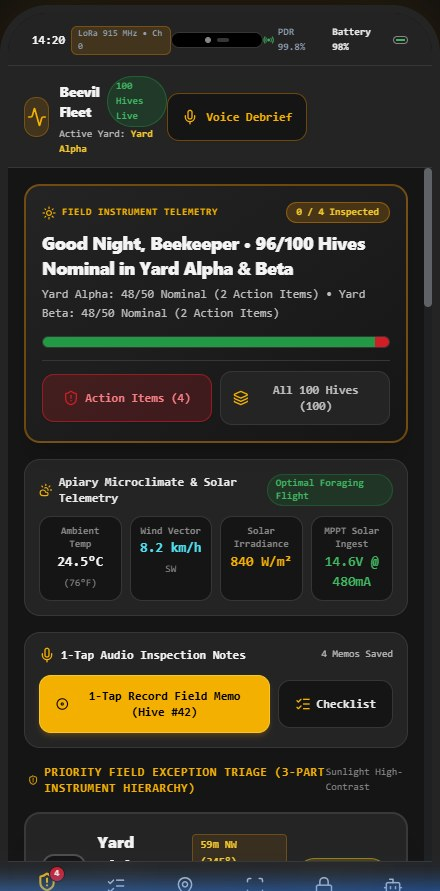
\includegraphics[width=0.31\textwidth]{figs/ui_field_console.jpg}}
\caption{Operator interfaces (DEMO mode, synthetic data): (a) companion PWA with inspection queue; (b) per-hive exception triage with the telemetry evidence behind an alert; (c) field console with apiary micro-climate.}
\label{fig:ui}
\end{figure*}

\begin{table}[!b]
\caption{Implementation Status and Evidence Class}
\label{tab:status}
\centering
\footnotesize
\begin{tabular}{@{}>{\raggedright\arraybackslash}p{2.55cm}>{\raggedright\arraybackslash}p{4.35cm}c@{}}
\toprule
Subsystem & Status & Class\\
\midrule
33-byte telemetry contract & implemented on node and gateway; unit-tested & \evT\\
Node firmware (bench) & compiles; reads on-chip temperature and battery ADC; external sensors auto-discovered but not yet populated & \evT/\evP\\
Node LoRa transmission & v1.0 transmitter emits a timing placeholder (LED and \SI{60}{ms} delay); radio driver integration pending & \evP\\
Acoustic band engine & Python reference, tested on synthetic tones; CMSIS-DSP port~\cite{cmsisdsp} pending & \evT/\evP\\
Gateway ingest, rules, SQLite, WebSocket & implemented; integration-tested & \evT\\
Gateway radio daemon & SPI receive loop is a stub; installed HAT is UART-based & \evP\\
Advisory Random Forest & trained and evaluated on synthetic data only & \evT\\
Multi-hop mesh & gateway router tested; node relaying not deployed & \evT/\evP\\
Operator interfaces & implemented; DEMO data & \evD\\
Radio, energy, CUSUM, acoustic studies & this paper (Section~\ref{sec:results}) & \evA\\
ANSYS models & four solved, one set up, one needs a port fix & \evS\\
Field deployment & not yet performed; 5-hive pilot planned & \evP\\
\bottomrule
\end{tabular}
\end{table}

% ===========================================================================
\section{Evaluation Methods}\label{sec:methods}
% ===========================================================================
\subsection{Evidence Classes and Provenance}\label{sec:m-evidence}
Every record carries a provenance tag: \texttt{REAL\_SENSOR}, \texttt{REAL\_SILICON} (on-chip temperature and battery ADC), \texttt{NOT\_CONNECTED}, \texttt{SIMULATED}, \texttt{SYNTHETIC} (test vectors) or \texttt{MANUAL\_TEST}. In this paper we also label every result as tested (\evT: executed code with assertions or benchmarks), analysed (\evA: analytical or Monte-Carlo models with stated assumptions), simulated (\evS: commercial multiphysics solvers), demonstrated (\evD: working interface on synthetic data) or planned (\evP). Table~\ref{tab:status} applies these labels to every subsystem.

\subsection{Software Verification and Gateway Benchmark}\label{sec:m-sw}
We executed the repository's pytest suite and its two self-contained benchmarks in a clean environment (Python 3.13, scikit-learn 1.9, two virtual CPUs of an Intel Xeon at \SI{2.8}{GHz}). For ingestion we started the gateway with Uvicorn on the loop-back interface in DEMO mode and posted 1000 frames (100 hives $\times$ 10 rounds) sequentially over one persistent HTTP/1.1 connection in each of five independent runs with a fresh database, using the repository's 100-hive generator, which injects a swarm signature (hive 12), brood chilling (hive 45) and a \SI{26}{\degree} knock-down (hive 88). To test cross-tier consistency, we also packed frames whose tilt byte carries the firmware alert flags and passed them through the gateway's unpacker and API.

\subsection{Radio Model}\label{sec:m-radio}
The time on air of a LoRa frame with a payload of $L$ bytes is~\cite{semtech2013an}
\begin{equation}
T_\mathrm{pkt} = \left(N_\mathrm{pre} + 4.25 + N_\mathrm{pl}\right) T_\mathrm{sym},\qquad T_\mathrm{sym} = 2^{\mathrm{SF}}/B,
\label{eq:toa}
\end{equation}
\begin{equation}
N_\mathrm{pl} = 8 + \max\!\left(\left\lceil \frac{8L - 4\,\mathrm{SF} + 44 - 20\,\mathrm{IH}}{4(\mathrm{SF} - 2\,\mathrm{DE})} \right\rceil (\mathrm{CR}+4),\,0\right),
\label{eq:npl}
\end{equation}
with $N_\mathrm{pre} = 8$, CRC enabled, explicit header ($\mathrm{IH}=0$), coding rate 4/5 ($\mathrm{CR}=1$), $B = \SI{125}{kHz}$ and low-data-rate optimisation $\mathrm{DE}=1$ for $\mathrm{SF}\geq 11$. For $N$ unsynchronised nodes reporting every $T$ seconds on $C$ channels, pure ALOHA~\cite{abramson1970} gives the delivery probability
\begin{equation}
\mathrm{PDR} = \exp\!\left(-2\,(N-1)\,T_\mathrm{pkt}/(C\,T)\right),
\label{eq:aloha}
\end{equation}
which neglects the capture effect and is therefore conservative; we cross-checked \eqref{eq:aloha} with an event-driven simulation of periodic nodes with $\pm$10\% jitter over \SI{24}{h}. The received power is $P_r = P_t + G_t - L_\mathrm{tx} - L_\mathrm{hive} + G_r - L_\mathrm{rx} - L_p(d)$ with $P_t = \SI{14}{dBm}$, $G_t = \SI{2.15}{dBi}$, $G_r = \SI{3}{dBi}$, $L_\mathrm{tx} = \SI{0.5}{dB}$, $L_\mathrm{rx} = \SI{1}{dB}$ and an assumed hive-body loss $L_\mathrm{hive} = \SI{8.7}{dB}$. The sensitivity $S = -174 + 10\log_{10}B + \mathrm{NF} + \mathrm{SNR}_\mathrm{min}(\mathrm{SF})$ with $\mathrm{NF} = \SI{6}{dB}$ reproduces the datasheet values of \SI{-124.5}{dBm} at SF7 and \SI{-137}{dBm} at SF12~\cite{sx1262ds}, and a \SI{15}{dB} fade margin is required. For the path loss $L_p$ we compare free space with the two-ray ground-reflection model~\cite{rappaport2002}
\begin{equation}
L_p(d) = 40\log_{10} d - 20\log_{10} (h_t h_r), \qquad d > d_c,
\label{eq:tworay}
\end{equation}
with $h_t = \SI{0.5}{m}$ (hive), $h_r = \SI{4}{m}$ (gateway mast) and breakpoint $d_c = 4\pi h_t h_r/\lambda = \SI{72}{m}$ (free space below $d_c$), and with \eqref{eq:tworay} plus Weissberger's foliage loss $L_f = 1.33 f^{0.284} d_f^{0.588}$~dB ($f$ in GHz, $14 < d_f \le \SI{400}{m}$)~\cite{weissberger1982,itur833} for $d_f = \SI{50}{m}$ of orchard canopy, i.e., \SI{12.7}{dB}.

\subsection{Energy Model}\label{sec:m-energy}
The charge drawn per reporting interval $T$ is $Q = I_\mathrm{sl}T + \sum_i I_i t_i$, and the autonomy (in days) of a cell of capacity $C_b$ with a self-discharge of $s$ per month is
\begin{equation}
L = \frac{C_b}{24\left(Q/T + C_b\, s/720\right)},
\label{eq:life}
\end{equation}
Table~\ref{tab:energy} lists the component currents and durations, taken as datasheet typical values~\cite{scd4xds,ds18b20ds,bme688ds,hx711ds,inmp441ds,tmp117ds,rak4631ds}. The SCD41 average of \SI{0.45}{mA} for one single-shot measurement every \SI{5}{min}~\cite{scd4xds} is consistent with a \SI{5}{s} acquisition at about \SI{18}{mA} plus idle current, so we model a power-gated single shot as \SI{90}{mA.s}. The transmit current of \SI{92}{mA} is the module value at \SI{+17}{dBm}~\cite{rak4631ds}, an upper bound for \SI{+14}{dBm} operation. We compare Policy~A (all sensors every \SI{5}{min}), Policy~B (\COtwo{} every \SI{30}{min} with the sensor power-gated) and Policy~C (no \COtwo{} sensor), with $s = 2\%$ per month.

\subsection{Brood-Cooling Change Detection}\label{sec:m-cusum}
Page's lower one-sided CUSUM with target $\mu_0 = \SI{34.82}{\celsius}$, reference value $k$ and threshold $h$ is~\cite{page1954,montgomery2013}
\begin{equation}
S_n = \max\!\left(0,\ S_{n-1} + (\mu_0 - T_n) - k\right), \qquad \text{alarm if } S_n \geq h.
\label{eq:page}
\end{equation}
The firmware variant latches the baseline $\hat\mu$ to the third sample after boot and decays the statistic at half rate,
\begin{equation}
S_n = \begin{cases} S_{n-1} + d_n, & d_n > 0\\ \max(0,\ S_{n-1} + d_n/2), & d_n \le 0\end{cases},\quad d_n = \hat\mu - T_n - k,
\label{eq:fw}
\end{equation}
with $k = \SI{0.15}{\celsius}$ and $h = 1.2$. Because $S_n$ accumulates once per sample, $h$ is in \si{\celsius}$\cdot$sample (\SI{0.1}{\celsius.h} at \SI{5}{min} sampling), not \si{\celsius.h} as documented. We model the regulated brood temperature as $T_n = \mu_0 + A\sin(2\pi n/288 + \phi) + e_n$, with AR(1) noise $e_n = \rho e_{n-1} + w_n$ of stationary standard deviation $\sigma = \SI{0.15}{\celsius}$ sampled every \SI{5}{min}, and consider an i.i.d.\ case ($\rho = 0$, $A = 0$), an autocorrelated case ($\rho = 0.9$) and an autocorrelated case with a diurnal component ($A = \SI{0.2}{\celsius}$). We estimate the probability of a false alarm within 30 days from 1000 runs, the in-control average run length $\mathrm{ARL}_0$ from 400 runs of 60 days (censored), and the median detection delay for step drops of \SIrange{0.3}{3.8}{\celsius} and ramps of \SIrange{0.02}{0.1}{\celsius\per\hour} after two in-control days (400 runs each).

\subsection{Acoustic Band Energy}\label{sec:m-acoustic}
The repository's decision engine computes, for each band $b$ with probe set $\mathcal{F}_b$ (5 to 7 frequencies),
\begin{equation}
E_b = \frac{1}{|\mathcal{F}_b|}\sum_{f\in\mathcal{F}_b}\left|\sum_{n=0}^{999} x[n]\, e^{-j2\pi f n/f_s}\right|
\label{eq:probe}
\end{equation}
over the first 1000 samples (\SI{62.5}{ms} at \SI{16}{kHz}), selects the dominant band and declares the colony normal if $\max_b E_b < 5$ (an absolute threshold). We re-implemented \eqref{eq:probe} (relative deviation from the reference code below $10^{-13}$) and compared it with a Hann-windowed Welch estimator that integrates the power of all FFT bins in each band~\cite{harris1978,welch1967},
\begin{equation}
P_b = \frac{1}{\sum_n w^2[n]}\sum_{k:\,f_k\in b}\big\langle |X_m[k]|^2 \big\rangle_m,
\label{eq:fft}
\end{equation}
with $N_\mathrm{FFT} = 2048$ and 50\% overlap over \SI{1}{s}. Test signals are three-harmonic tones (relative amplitudes 0.6, 0.3, 0.1) whose fundamental is drawn uniformly inside one of the bands \SIrange{100}{180}{Hz}, \SIrange{200}{400}{Hz}, \SIrange{450}{750}{Hz} or \SIrange{800}{1200}{Hz}, with 60 trials per band and condition. The noise is Gaussian and band-limited to \SIrange{50}{1500}{Hz} so that it overlaps every band. Accuracy is the fraction of trials whose dominant band equals the true band.

\subsection{Gateway Advisory Classifier}\label{sec:m-rf}
The advisory model is a Random Forest~\cite{breiman2001,pedregosa2011} (100 trees, depth 8) over four features: brood temperature, dominant acoustic frequency, \COtwo{} and hive mass, trained on 1500 samples drawn from class-conditional Gaussians whose parameters follow published ranges (healthy 1051, swarming 138, starvation 158, queenless 153). We report stratified five-fold cross-validation, robustness to additive Gaussian perturbations scaled to the healthy-class standard deviations (\SI{0.5}{\celsius}, \SI{40}{Hz}, \SI{150}{ppm}, \SI{2.5}{kg}), and single-sensor drop-out in which one feature is replaced by its healthy-class median.

\subsection{Multiphysics Models}\label{sec:m-sim}
The repository contains ANSYS models built with ANSYS Student 2026 R1 (Mechanical, SPEOS) and Electronics Desktop Student 2025 R2.4 (HFSS). Simulation files and model geometry are preserved in the repository (\url{https://github.com/atharveeee-netizen/beevil-knievel/tree/main/hardware/simulations}). We report only the models whose solutions are documented by a solver log or by a screenshot of the solver interface (Table~\ref{tab:ansys}).

% ===========================================================================
\section{Results}\label{sec:results}
% ===========================================================================
\subsection{Software Verification, Ingestion Performance and a Cross-Tier Defect}\label{sec:r-sw}
All 29 tests pass in \SI{2.4}{s} (Table~\ref{tab:verif}). The acoustic stress benchmark classifies 30 of 30 synthetic tones and the advisory benchmark 4 of 4 scenarios, as published. The real-audio benchmarks on the Zenodo recordings~\cite{nolasco2018data} could not be re-executed because the dataset host was not reachable from our build environment. In the published three-clip evaluation, moreover, the queenless clips are paired with a \SI{4}{\celsius} brood-to-ambient difference, which triggers the thermal rule regardless of the audio, so that test does not isolate acoustic performance.

Over five runs of 1000 frames the gateway sustained a median of 299 frames/s (range 265 to 336); the median values of the mean, 50th-, 95th- and 99th-percentile latencies were 3.26, 3.10, 4.96 and \SI{7.10}{ms}, and the 99th percentile never exceeded \SI{8.1}{ms}. It routed the three injected anomalies to \texttt{PRE\_SWARM\_WARNING}, \texttt{THERMAL\_STRESS} and \texttt{TAMPER\_THEFT} and reported every other hive as healthy. A 100-hive apiary reporting every \SI{5}{min} offers \SI{0.33}{frames/s}, so even a 50-fold slower single-board computer would keep a margin above 15 (the Raspberry Pi itself was not benchmarked).

The cross-tier test exposes a defect. The firmware ORs its alert flags (\texttt{0x80} CUSUM, \texttt{0x40} pre-swarm, \texttt{0x20} low battery, \texttt{0x10} tamper) into the tilt byte, whereas the gateway interprets that byte as degrees. A low-battery flag therefore reads as a \SI{33}{\degree} tilt and is diagnosed as theft, a pre-swarm flag (\SI{64}{\degree}) likewise, and the CUSUM queen-loss flag (\SI{129}{\degree}) violates the \SI{90}{\degree} schema bound, so the frame is rejected with HTTP 422 and the most critical alert is silently dropped. A dedicated flags byte plus an 8-bit sequence number (35 bytes) removes the ambiguity, enables loss accounting in star mode and costs \SI{5.1}{ms} of extra airtime at SF7 (\SI{77.1}{ms}).

\begin{table}[!t]
\caption{Reproduced Software Verification (\evT)}
\label{tab:verif}
\centering
\footnotesize
\setlength{\tabcolsep}{4pt}
\begin{tabular}{@{}>{\raggedright\arraybackslash}p{4.75cm}r@{}}
\toprule
Item & Result\\
\midrule
Telemetry contract and firmware arithmetic (struct layout, sentinels, CRC-16/CCITT, SoC table, CUSUM, FFT bin mapping, header consistency, serial-log parsing) & 18/18\\
Gateway pipeline (REST, schema rejection, anomaly routing, alert persistence, binary unpack end-to-end, mesh de-duplication) & 8/8\\
Advisory model interface & 3/3\\
\midrule
Acoustic stress benchmark (noise-free tones) & 30/30\\
Advisory scenario benchmark & 4/4\\
Zenodo real-audio benchmarks & not re-run\\
\midrule
Ingestion, median (range) of 5 runs & 299 (265 to 336) frames/s\\
Latency mean/p50/p95/p99, median (ms) & 3.26/3.10/4.96/7.10\\
Injected anomalies correctly routed & 3/3\\
Flags in tilt byte: low battery, pre-swarm, CUSUM & theft, theft, HTTP 422\\
\bottomrule
\end{tabular}
\end{table}

\subsection{Radio Link and Medium Access (\evA)}\label{sec:r-radio}
Table~\ref{tab:lora} and Fig.~\ref{fig:lora} summarise the radio analysis. The 33-byte frame needs 58 payload symbols and \SI{71.9}{ms} at SF7, a per-node duty cycle of 0.024\% at \SI{5}{min} reporting; airtime roughly doubles with every SF step and reaches \SI{1.81}{s} at SF12. The IN865 band imposes no duty-cycle limit~\cite{lorawanrp,actility2025}, so the binding constraints are collisions and energy rather than regulation. Under pure ALOHA a single channel delivers 95.4\% of frames for 100 hives at SF7 (event-driven simulation: 95.1\%); 99\% delivery is reached only up to 21 hives (63 with three channels), and at SF10 delivery falls to 74.2\%. A 100-hive yard therefore needs several channels, acknowledged retransmission or, because the gateway is powered and can transmit a beacon, time-slotted reporting keyed to the hive identifier. A \SI{300}{s} period holds more than 4000 slots of \SI{72}{ms}, enough for collision-free operation with guard intervals that absorb a 20-ppm crystal drift (\SI{6}{ms} per period).

Range is governed by antenna height. With the hive antenna at \SI{0.5}{m} and the gateway antenna at \SI{4}{m}, the first Fresnel zone at the mid-point of a \SI{1}{km} link has a radius of \SI{9.3}{m}, so ground reflection dominates beyond \SI{72}{m}. Free-space loss would predict \SI{23}{km} at SF7 and is the origin of the \SI{15}{km} figures in earlier project documents; the two-ray model gives \SI{1.30}{km}, and \SI{50}{m} of orchard canopy reduces this to \SI{0.62}{km}. SF12 extends these to \SI{2.66}{km} and \SI{1.28}{km} at 25 times the airtime and transmit energy (\SI{550}{mJ} versus \SI{21.8}{mJ} per frame). The analysis agrees with the project's own field estimate of \SIrange{1.0}{1.5}{km} and shows that raising the gateway antenna is more effective than raising SF: doubling $h_r$ adds \SI{6}{dB}, worth more than two SF steps.

\begin{table*}[!t]
\caption{LoRa Analysis for the 33-Byte Frame (BW \SI{125}{kHz}, CR 4/5, $T = \SI{300}{s}$, \SI{15}{dB} Fade Margin) (\evA)}
\label{tab:lora}
\centering
\footnotesize
\setlength{\tabcolsep}{4.4pt}
\begin{tabular}{@{}cccccccccccc@{}}
\toprule
 & ToA & Payload & Sensitivity & Max.\ path & \multicolumn{3}{c}{Range (km)} & TX energy & \multicolumn{2}{c}{PDR at $N=100$ (\%)} & Max.\ $N$ at 99\%\\
\cmidrule(lr){6-8}\cmidrule(lr){10-11}
SF & (ms) & symbols & (dBm) & loss (dB) & free space & two-ray & two-ray + foliage & (mJ) & 1 channel & 3 channels & (1 / 3 channels)\\
\midrule
7  & 71.9   & 58 & $-124.5$ & 118.5 & 23.1 & 1.30 & 0.62 & 21.8  & 95.4 & 98.4 & 21 / 63\\
8  & 133.6  & 53 & $-127.0$ & 121.0 & 30.8 & 1.49 & 0.72 & 40.6  & 91.6 & 97.1 & 12 / 34\\
9  & 246.8  & 48 & $-129.5$ & 123.5 & 41.1 & 1.72 & 0.83 & 74.9  & 85.0 & 94.7 & 7 / 19\\
10 & 452.6  & 43 & $-132.0$ & 126.0 & 54.8 & 1.99 & 0.96 & 137.4 & 74.2 & 90.5 & 4 / 10\\
11 & 987.1  & 48 & $-134.5$ & 128.5 & 73.1 & 2.30 & 1.11 & 299.7 & 52.1 & 80.5 & 2 / 5\\
12 & 1810.4 & 43 & $-137.0$ & 131.0 & 97.5 & 2.66 & 1.28 & 549.6 & 30.3 & 67.2 & 1 / 3\\
\bottomrule
\end{tabular}
\end{table*}

\begin{figure*}[!t]
\centering
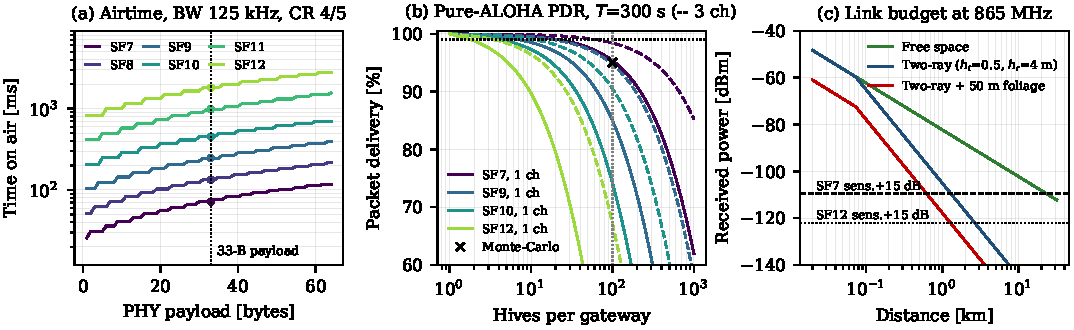
\includegraphics[width=\textwidth]{figs/fig_lora.pdf}
\caption{Radio analysis (\evA). (a) Airtime versus payload; dots mark the 33-byte frame. (b) Pure-ALOHA delivery versus hives per gateway for one (solid) and three (dashed) channels; the cross is the event-driven simulation for SF7. (c) Received power versus distance for free space, the two-ray model and two-ray plus \SI{50}{m} of foliage, against SF7 and SF12 sensitivity plus the fade margin.}
\label{fig:lora}
\end{figure*}

\subsection{Node Energy Budget (\evA)}\label{sec:r-energy}
Table~\ref{tab:energy} and Fig.~\ref{fig:energy} give the budget. With every sensor read every \SI{5}{min} (Policy~A), the node draws \SI{527}{\micro\ampere} on average, 85\% of it in the SCD41; a single \COtwo{} measurement costs about 14 times the charge of a LoRa frame. Autonomy on a \SI{2600}{mAh} cell is 206 days without self-discharge and 181 days with 2\% per month. Measuring \COtwo{} every \SI{30}{min} with the sensor power-gated (Policy~B) lowers the average to \SI{127}{\micro\ampere} and extends autonomy to 545 days; \COtwo{} (40\%), the radio (17\%) and audio capture (12\%) are then the largest consumers. Removing \COtwo{} altogether (Policy~C) gives \SI{77}{\micro\ampere} and 728 days. Even under Policy~A the \SI{0.6}{W} panel yields about \SI{97}{mAh} per day at one equivalent peak-sun hour (60\% charger efficiency), 7.7 times the daily need of \SI{12.6}{mAh}, so the node is energy-neutral unless the panel is persistently shaded. These figures exclude cold-temperature capacity loss and must be confirmed with a current profiler.

\begin{table}[!t]
\caption{Bottom-Up Charge per \SI{300}{s} Cycle (Datasheet Typical Values) (\evA)}
\label{tab:energy}
\centering
\footnotesize
\setlength{\tabcolsep}{3pt}
\resizebox{\columnwidth}{!}{%
\begin{tabular}{@{}llrr@{}}
\toprule
 & & \multicolumn{2}{c}{Charge (mA$\cdot$s)}\\
\cmidrule(l){3-4}
Component & Assumption & Pol.\ A & Pol.\ B\\
\midrule
Sleep floor & \SI{5}{\micro\ampere} (module \SI{2}{\micro\ampere}~\cite{rak4631ds} + board) & 1.50 & 1.50\\
SCD41 \COtwo{} & \SI{0.45}{mA} avg.; gated \SI{90}{mA.s}/shot & 135.00 & 15.00\\
5$\times$DS18B20 & \SI{1}{mA} $\times$ \SI{0.75}{s} each & 3.75 & 3.75\\
BME688 & \SI{12}{mA} $\times$ \SI{0.15}{s} (heater) & 1.80 & 1.80\\
HX711 + bridge & (1.5 + 3.0) mA $\times$ \SI{0.8}{s} & 3.60 & 3.60\\
Audio capture & (1.4 + 3.3) mA $\times$ \SI{1}{s} & 4.70 & 4.70\\
MCU housekeeping & \SI{3.3}{mA} $\times$ \SI{0.3}{s} & 0.99 & 0.99\\
TMP117 & \SI{135}{\micro\ampere} $\times$ \SI{15.5}{ms} & 0.002 & 0.002\\
LoRa frame (SF7) & \SI{92}{mA} $\times$ \SI{71.9}{ms} & 6.62 & 6.62\\
\midrule
Total / average current & & 158.0 / 527\,\si{\micro\ampere} & 38.0 / 127\,\si{\micro\ampere}\\
Autonomy, \SI{2600}{mAh} & no / 2\%-per-month self-discharge & 206 / 181\,d & 856 / 545\,d\\
\bottomrule
\end{tabular}}
\end{table}

\begin{figure*}[!t]
\centering
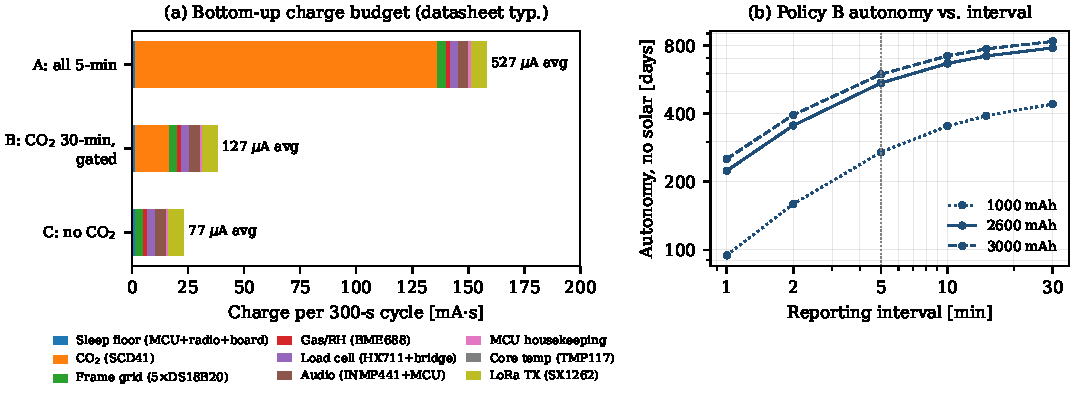
\includegraphics[width=0.92\textwidth]{figs/fig_energy.pdf}
\caption{Energy analysis (\evA). (a) Charge per \SI{300}{s} cycle by component for the three policies. (b) Policy-B autonomy without solar input versus reporting interval for three cell capacities (2\% per month self-discharge).}
\label{fig:energy}
\end{figure*}

\subsection{Brood-Cooling Change Detection (\evA)}\label{sec:r-cusum}
Table~\ref{tab:cusum} and Fig.~\ref{fig:cusum} summarise the detector study. Under i.i.d.\ variability the firmware detector already false-alarms within 30 days in 37\% of runs; with autocorrelated variability this rises to 86\%, and with an added diurnal component to 93\%, with a median time to the first false alarm of 0.41 day. Both the latched single-sample baseline and the half-rate decay contribute: Page's CUSUM with the same $k$ and $h$ false-alarms in only 0.1\% of i.i.d.\ runs. Autocorrelation is the dominant effect, because slow excursions accumulate in $S_n$ as if they were persistent shifts. Raising the reference value to $k = \SI{0.25}{\celsius}$ (half of a \SI{0.5}{\celsius} design shift) and the threshold to $h = 8$ gives $\mathrm{ARL}_0 = 34$ days in the hardest case. The re-tuned detector flags a \SI{1}{\celsius} drop after a median of \SI{0.92}{h}, a \SI{0.5}{\celsius} drop after \SI{2.5}{h} and the \SI{3.8}{\celsius} collapse used in the firmware unit test after \SI{15}{min}. For a gradual cooling of \SI{0.05}{\celsius\per\hour} the alarm comes after \SI{9.3}{h}, when the brood has cooled by about \SI{0.47}{\celsius} and is still inside its regulated range. The firmware detector looks faster in Table~\ref{tab:cusum}, but only in the 19 to 24\% of runs that had not already raised a false alarm before the change. Because $\mathrm{ARL}_0$ is very sensitive to $\rho$ and $\sigma$, $k$ and $h$ must be calibrated on field data; Fig.~\ref{fig:cusum}(b) is the corresponding design chart.

\begin{table}[!t]
\caption{CUSUM Detectors Under the Brood-Temperature Model (\evA)}
\label{tab:cusum}
\centering
\footnotesize
\setlength{\tabcolsep}{2.4pt}
\begin{tabular}{@{}lccc@{}}
\toprule
 & Firmware & Page & Page\\
 & $k$=0.15, $h$=1.2 & $k$=0.15, $h$=1.2 & $k$=0.25, $h$=8\\
\midrule
$P$(false alarm $\le$ 30 d), i.i.d. & 0.37 & 0.00 & 0.00\\
\quad AR(1), $\rho = 0.9$ & 0.86 & 1.00 & 0.00\\
\quad AR(1) + diurnal & 0.93 & 1.00 & 0.47\\
$\mathrm{ARL}_0$ (d), AR(1) + diurnal & 0.41$^{*}$ & 0.33$^{*}$ & 34\\
\midrule
Median delay (h): \SI{0.5}{\celsius} step & 0.46$^{\dagger}$ & --- & 2.46\\
\quad \SI{1.0}{\celsius} step & 0.17$^{\dagger}$ & --- & 0.92\\
\quad \SI{3.8}{\celsius} step & 0.08$^{\dagger}$ & --- & 0.25\\
\quad \SI{0.05}{\celsius\per\hour} ramp & 8.83$^{\dagger}$ & --- & 9.33\\
\bottomrule
\end{tabular}
\\[2pt]\parbox{\columnwidth}{\footnotesize $^{*}$Median run length. $^{\dagger}$Only runs without a prior false alarm (19 to 24\%); 76 to 81\% of firmware runs alarmed before the change.}
\end{table}

\begin{figure*}[!t]
\centering
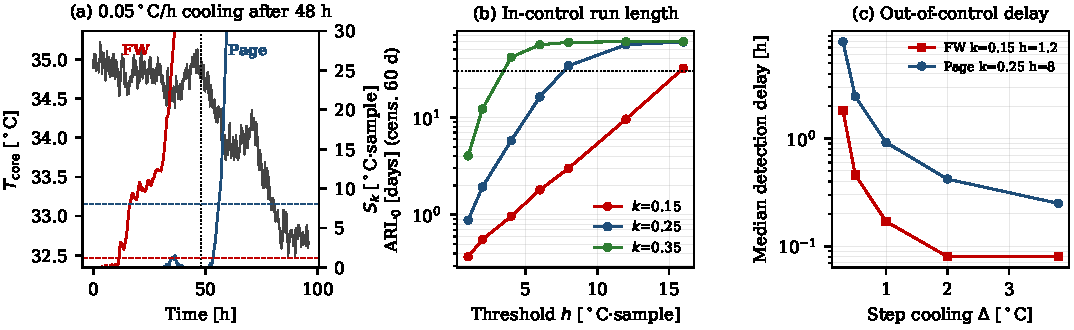
\includegraphics[width=\textwidth]{figs/fig_cusum_mc.pdf}
\caption{Brood-cooling CUSUM (\evA). (a) Example trace with a \SI{0.05}{\celsius\per\hour} cooling ramp from hour 48; the firmware statistic (red) crosses its threshold long before the change, the re-tuned Page statistic (blue) only after it. (b) In-control average run length versus threshold for three reference values (AR(1) + diurnal model; dotted line: 30 days). (c) Median detection delay versus step size (firmware: runs without a prior false alarm only).}
\label{fig:cusum}
\end{figure*}

\subsection{Acoustic Front End (\evA)}\label{sec:r-acoustic}
Fig.~\ref{fig:dsp} reproduces the repository's model-based DSP illustrations. With a Hann window and $\Delta f = \SI{7.81}{Hz}$, synthetic fanning (\SI{140}{Hz}), waggle-like (\SI{240}{Hz}) and piping (\SI{340}{Hz}) components are cleanly separated; a pair of tones \SI{20}{Hz} apart (235 and \SI{255}{Hz}) is resolved with sidelobes about \SI{32}{dB} down instead of \SI{13}{dB} for a rectangular window; and band-energy trajectories respond within one frame to a simulated pre-swarm onset.

The robustness audit (Fig.~\ref{fig:acoustic}) shows where the deployed estimator departs from this ideal. Because \eqref{eq:probe} samples only 5 to 7 discrete frequencies per band with a \SI{62.5}{ms} window whose main lobe is \SI{\pm16}{Hz} wide, its band response ripples by 3.4, 14.0, 16.4 and \SI{23.3}{dB} within the four bands, against at most \SI{0.4}{dB} for \eqref{eq:fft}, so tones that fall between probes are attenuated. With band-limited noise the probe engine's dominant-band accuracy is 94 to 95\% at \SIrange{10}{30}{dB} SNR and 71\% at \SI{0}{dB}, while FFT integration stays at 100\% down to \SI{0}{dB} and 97\% at \SI{-5}{dB}. More importantly, the absolute decision threshold makes the probe engine gain-dependent: its accuracy falls from 90\% at \SI{-6}{dBFS} to chance (25\%) at \SI{-24}{dBFS} and below, whereas a decision on relative band energies is level-invariant by construction. The same effect is visible in Fig.~\ref{fig:dsp}(f), where no band trajectory reaches the illustrated absolute threshold $\tau = 0.12$.

Table~\ref{tab:dsp} relates the implemented and documented front-end configurations. 256 points at \SI{16}{kHz} resolve the \SIrange{100}{180}{Hz} fanning band with a single bin, while 256 points at \SI{2}{kHz} alias the \SIrange{800}{1200}{Hz} noise band. Decimating the \SI{16}{kHz} I$^2$S stream by four and using a 512-point FFT gives \SI{7.81}{Hz} resolution, covers all four bands with 11 to 51 bins each and needs only \SI{4}{kB} of buffer memory. We recommend this configuration, together with relative band energies and a separate, calibrated loudness gate.

\begin{figure*}[!t]
\centering
\subfloat[]{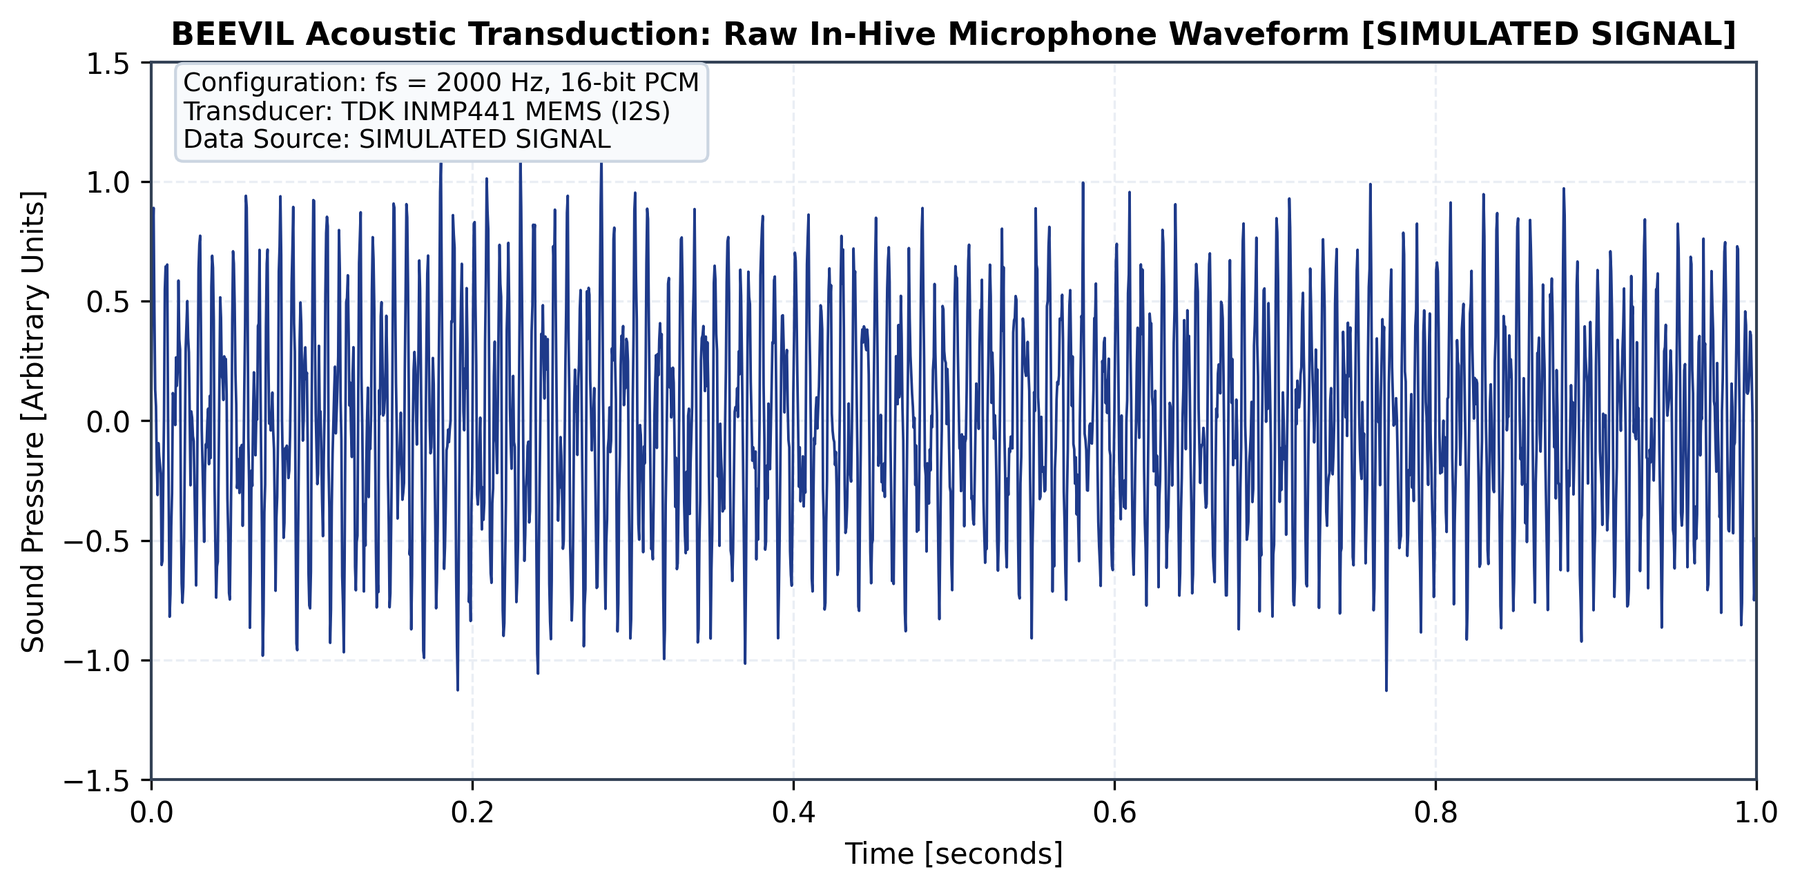
\includegraphics[width=0.318\textwidth]{figs/repo_acoustic_raw_signal.png}}\hfil
\subfloat[]{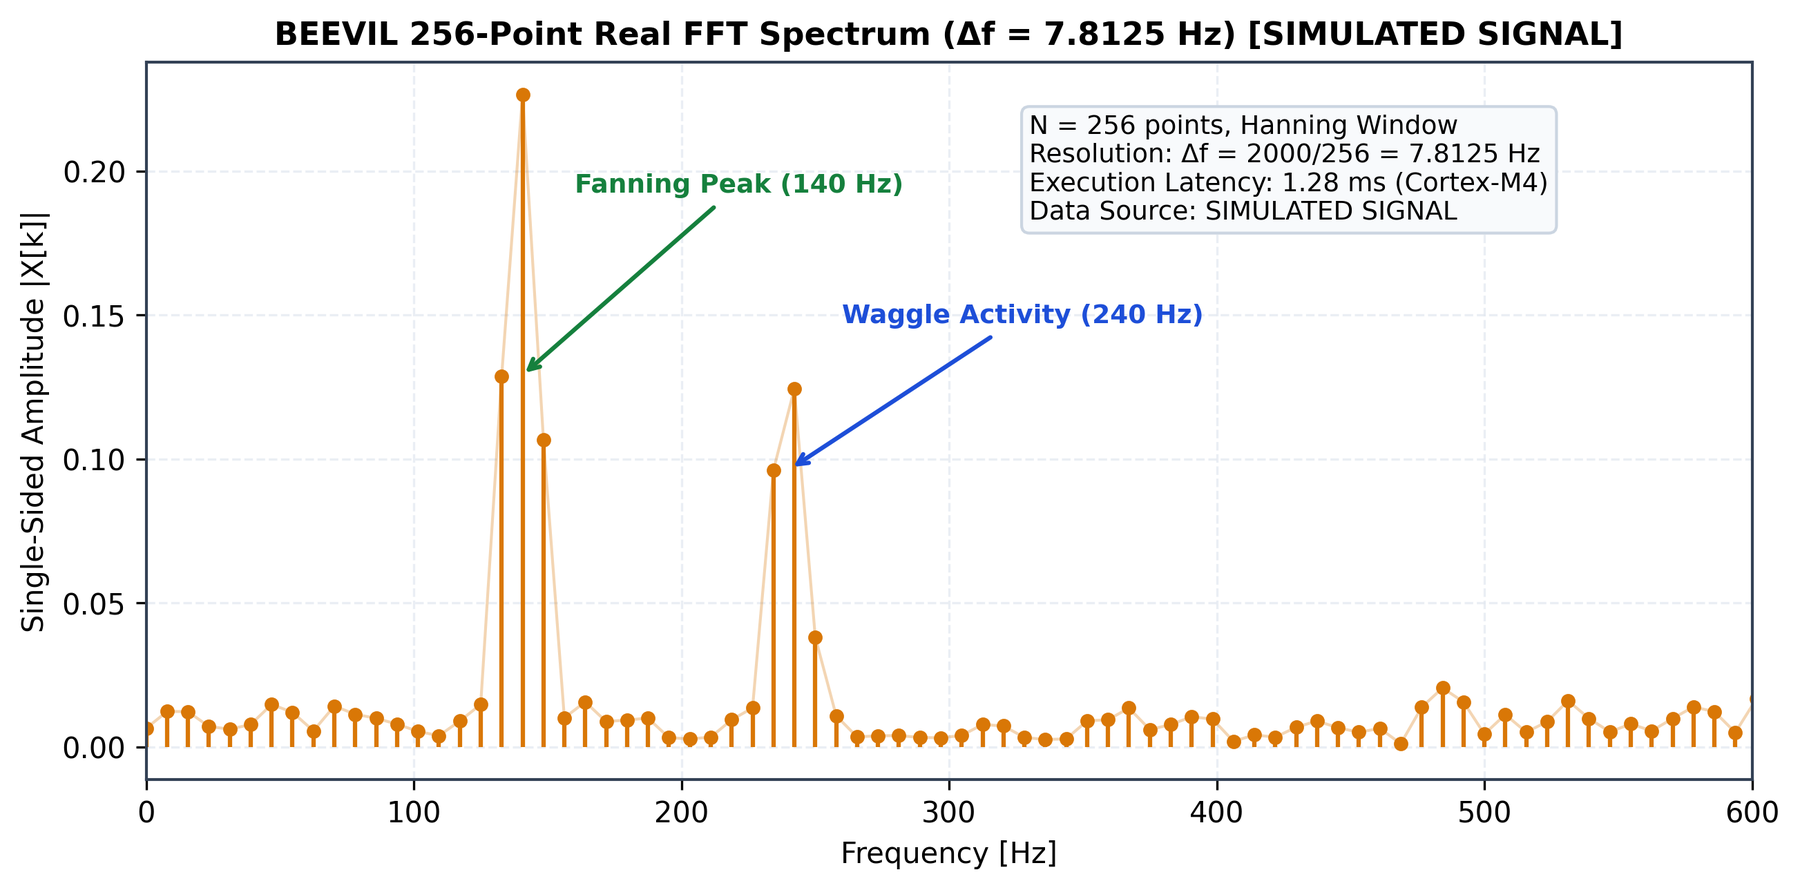
\includegraphics[width=0.318\textwidth]{figs/repo_acoustic_fft.png}}\hfil
\subfloat[]{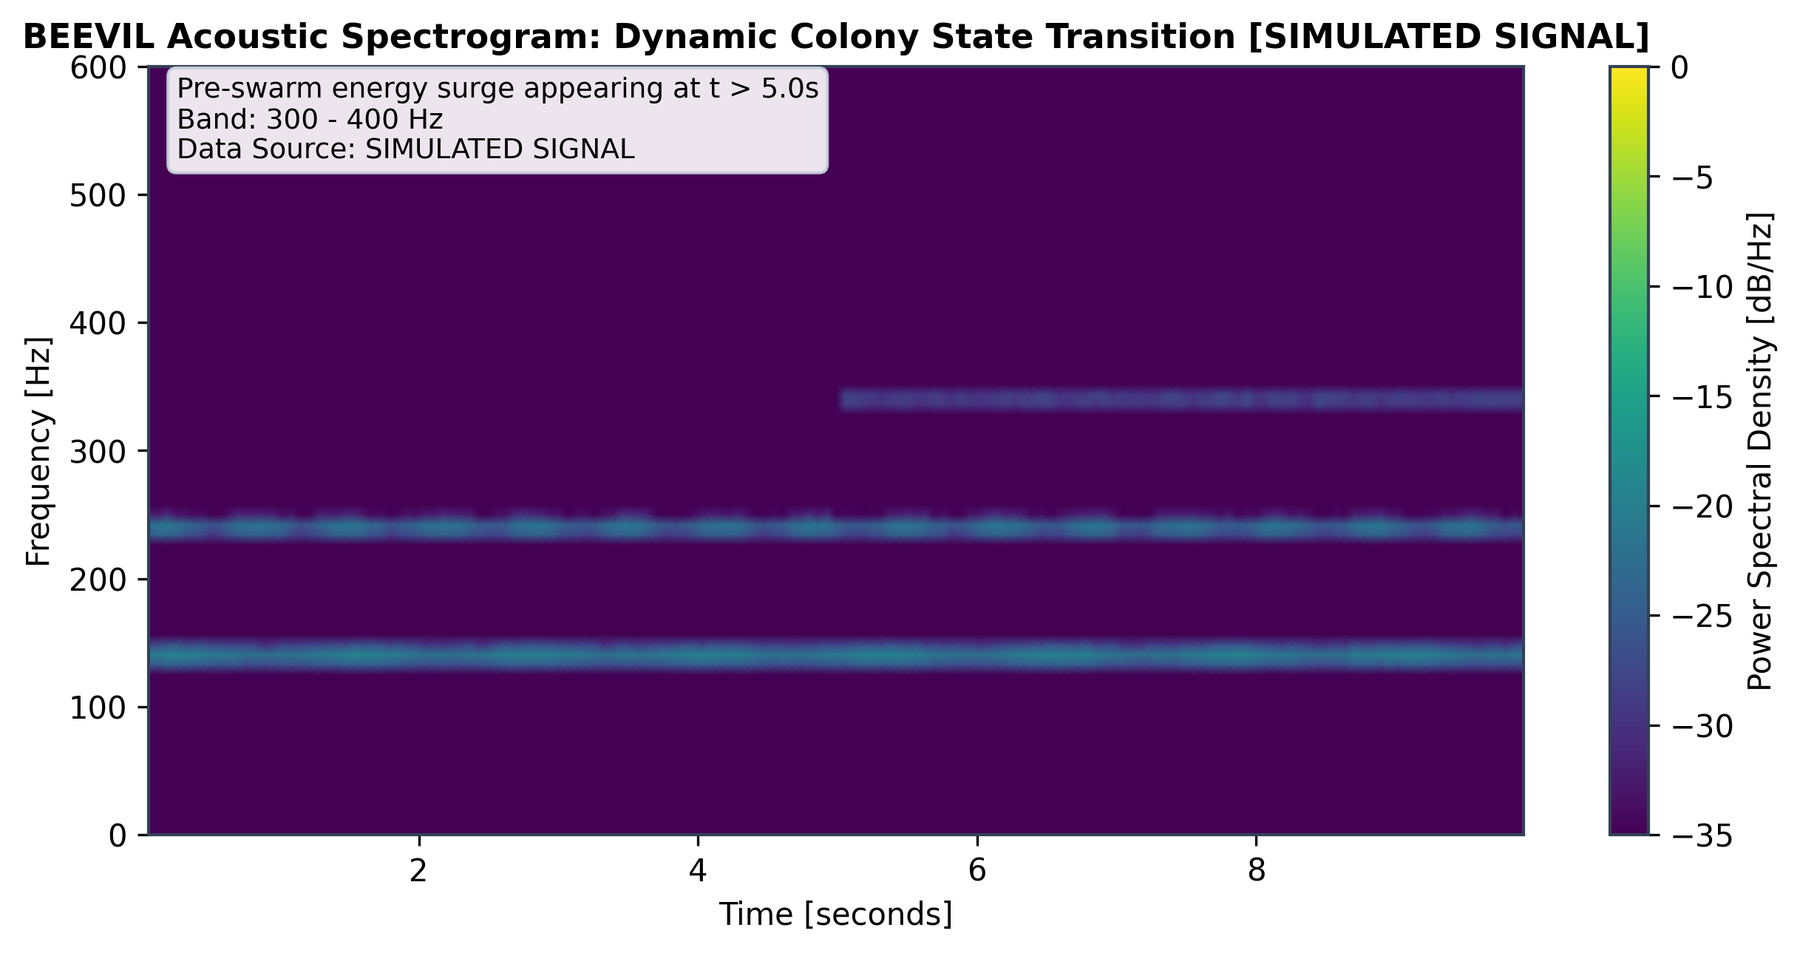
\includegraphics[width=0.318\textwidth]{figs/repo_acoustic_spectrogram.png}}\\[-1pt]
\subfloat[]{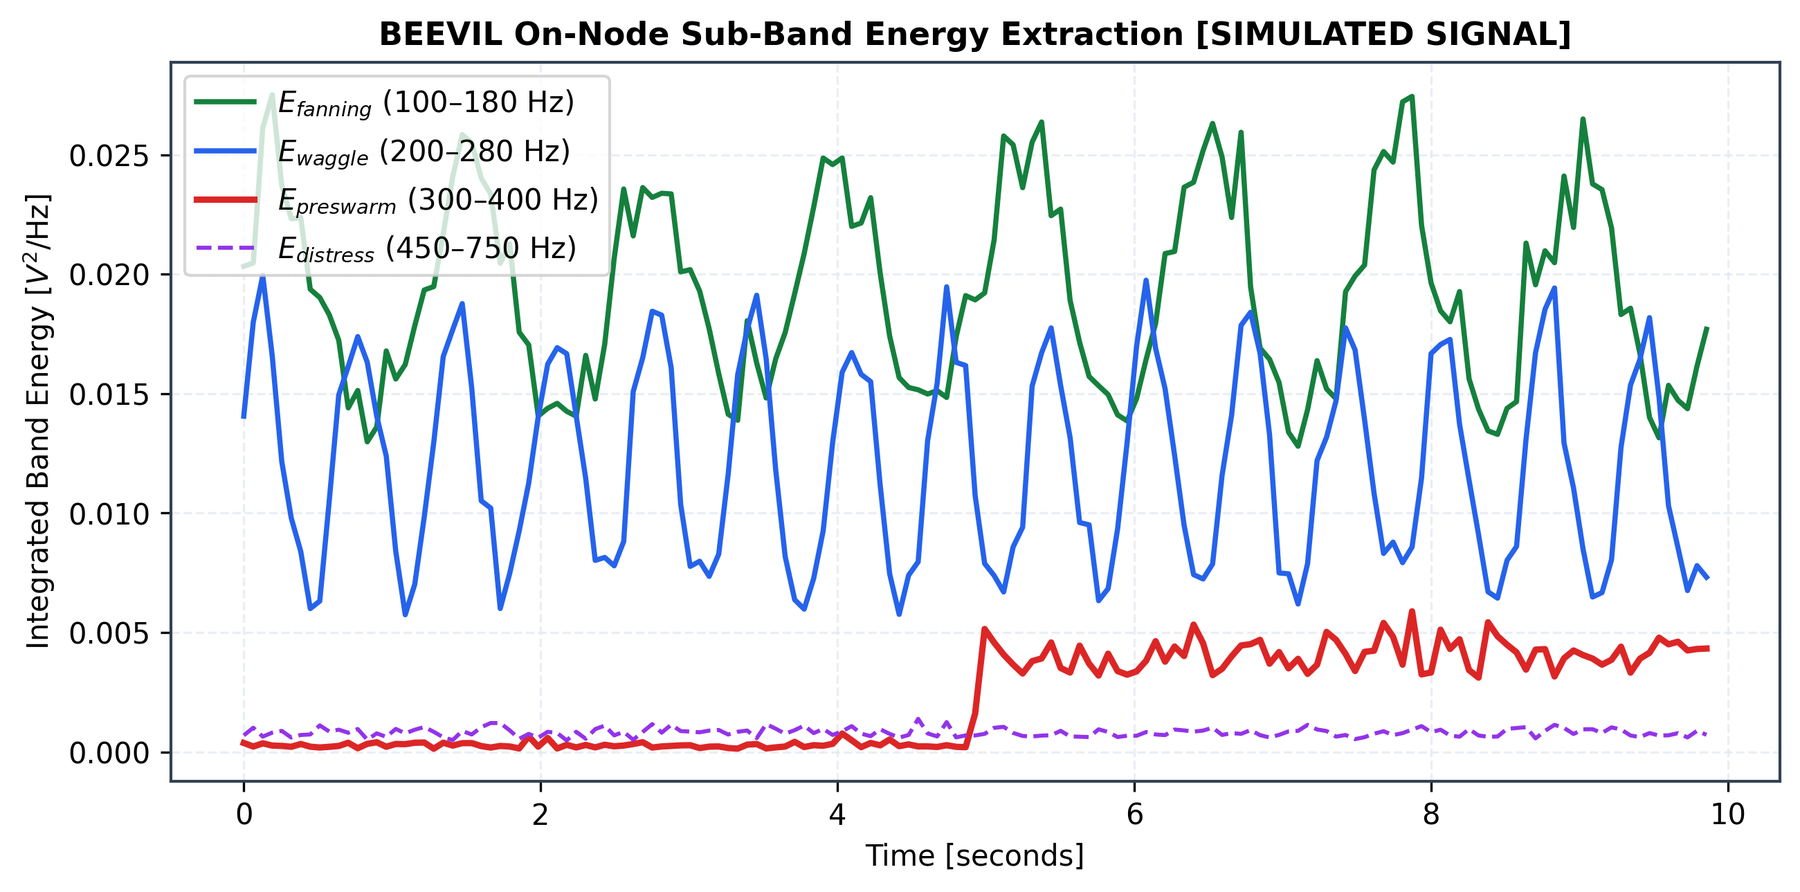
\includegraphics[width=0.318\textwidth]{figs/repo_acoustic_features.png}}\hfil
\subfloat[]{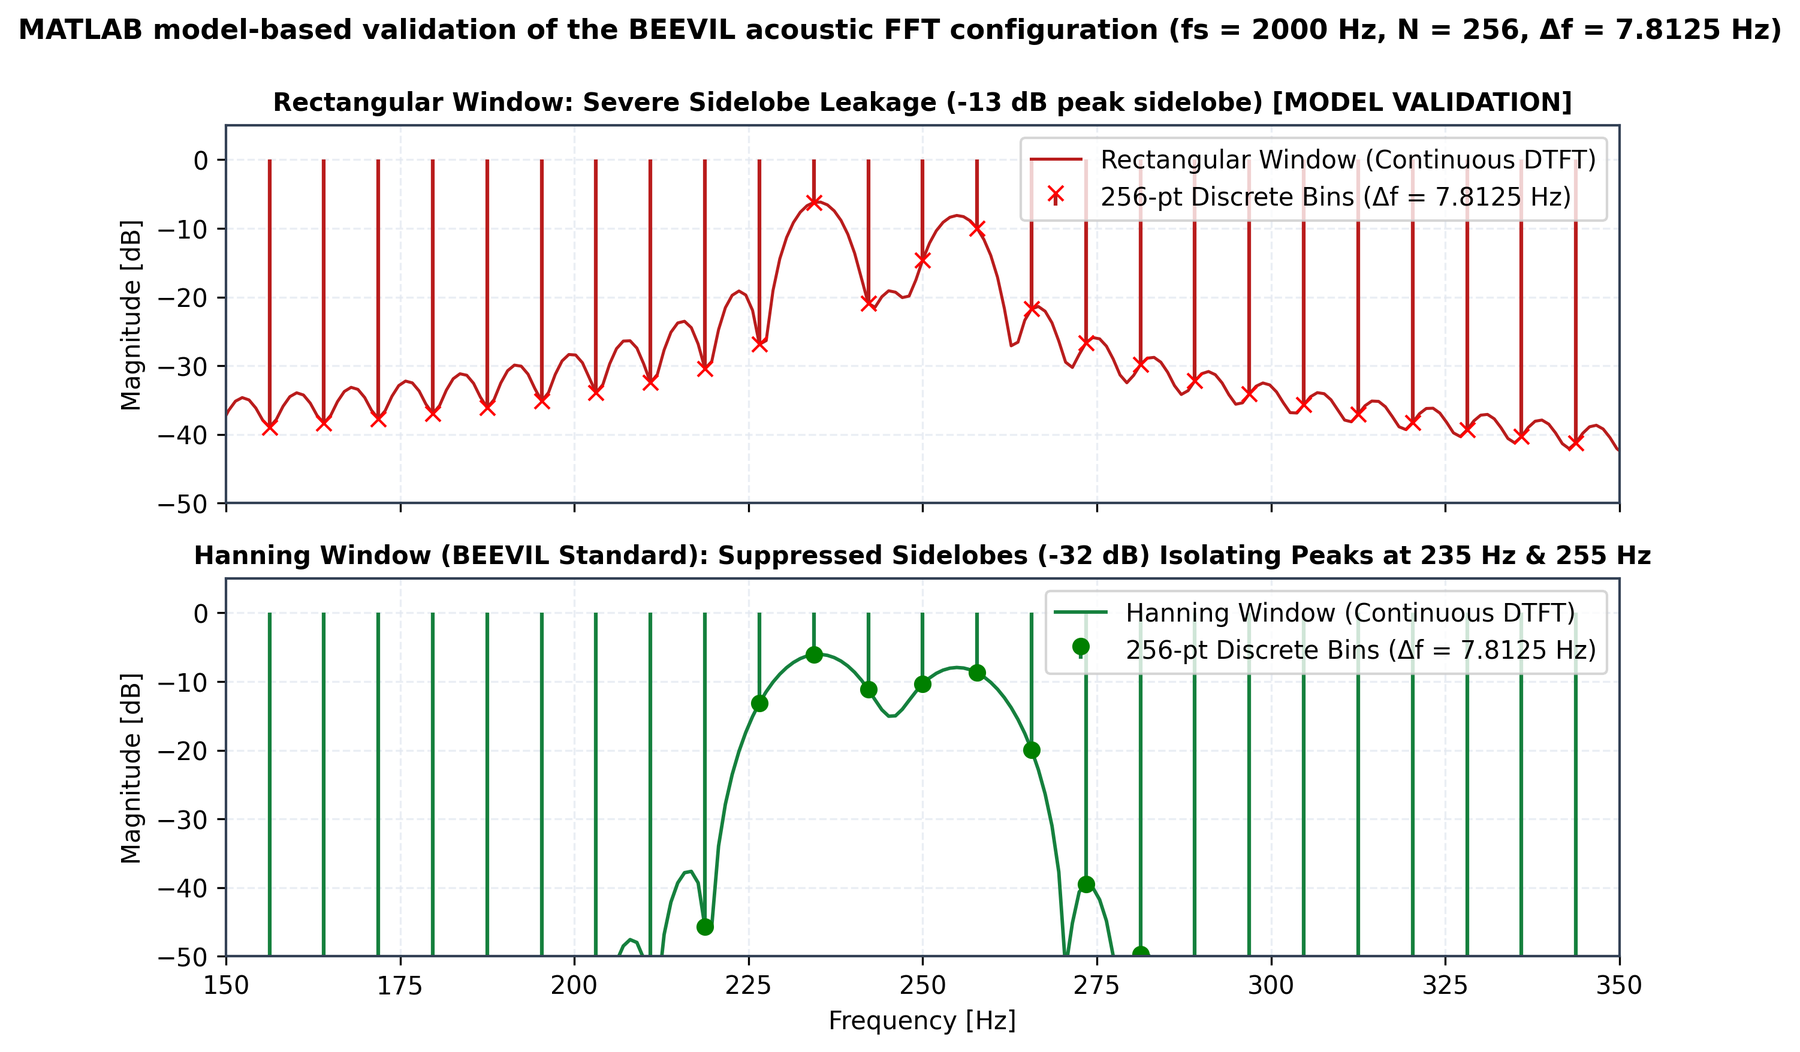
\includegraphics[width=0.318\textwidth]{figs/repo_fft_resolution_validation.png}}\hfil
\subfloat[]{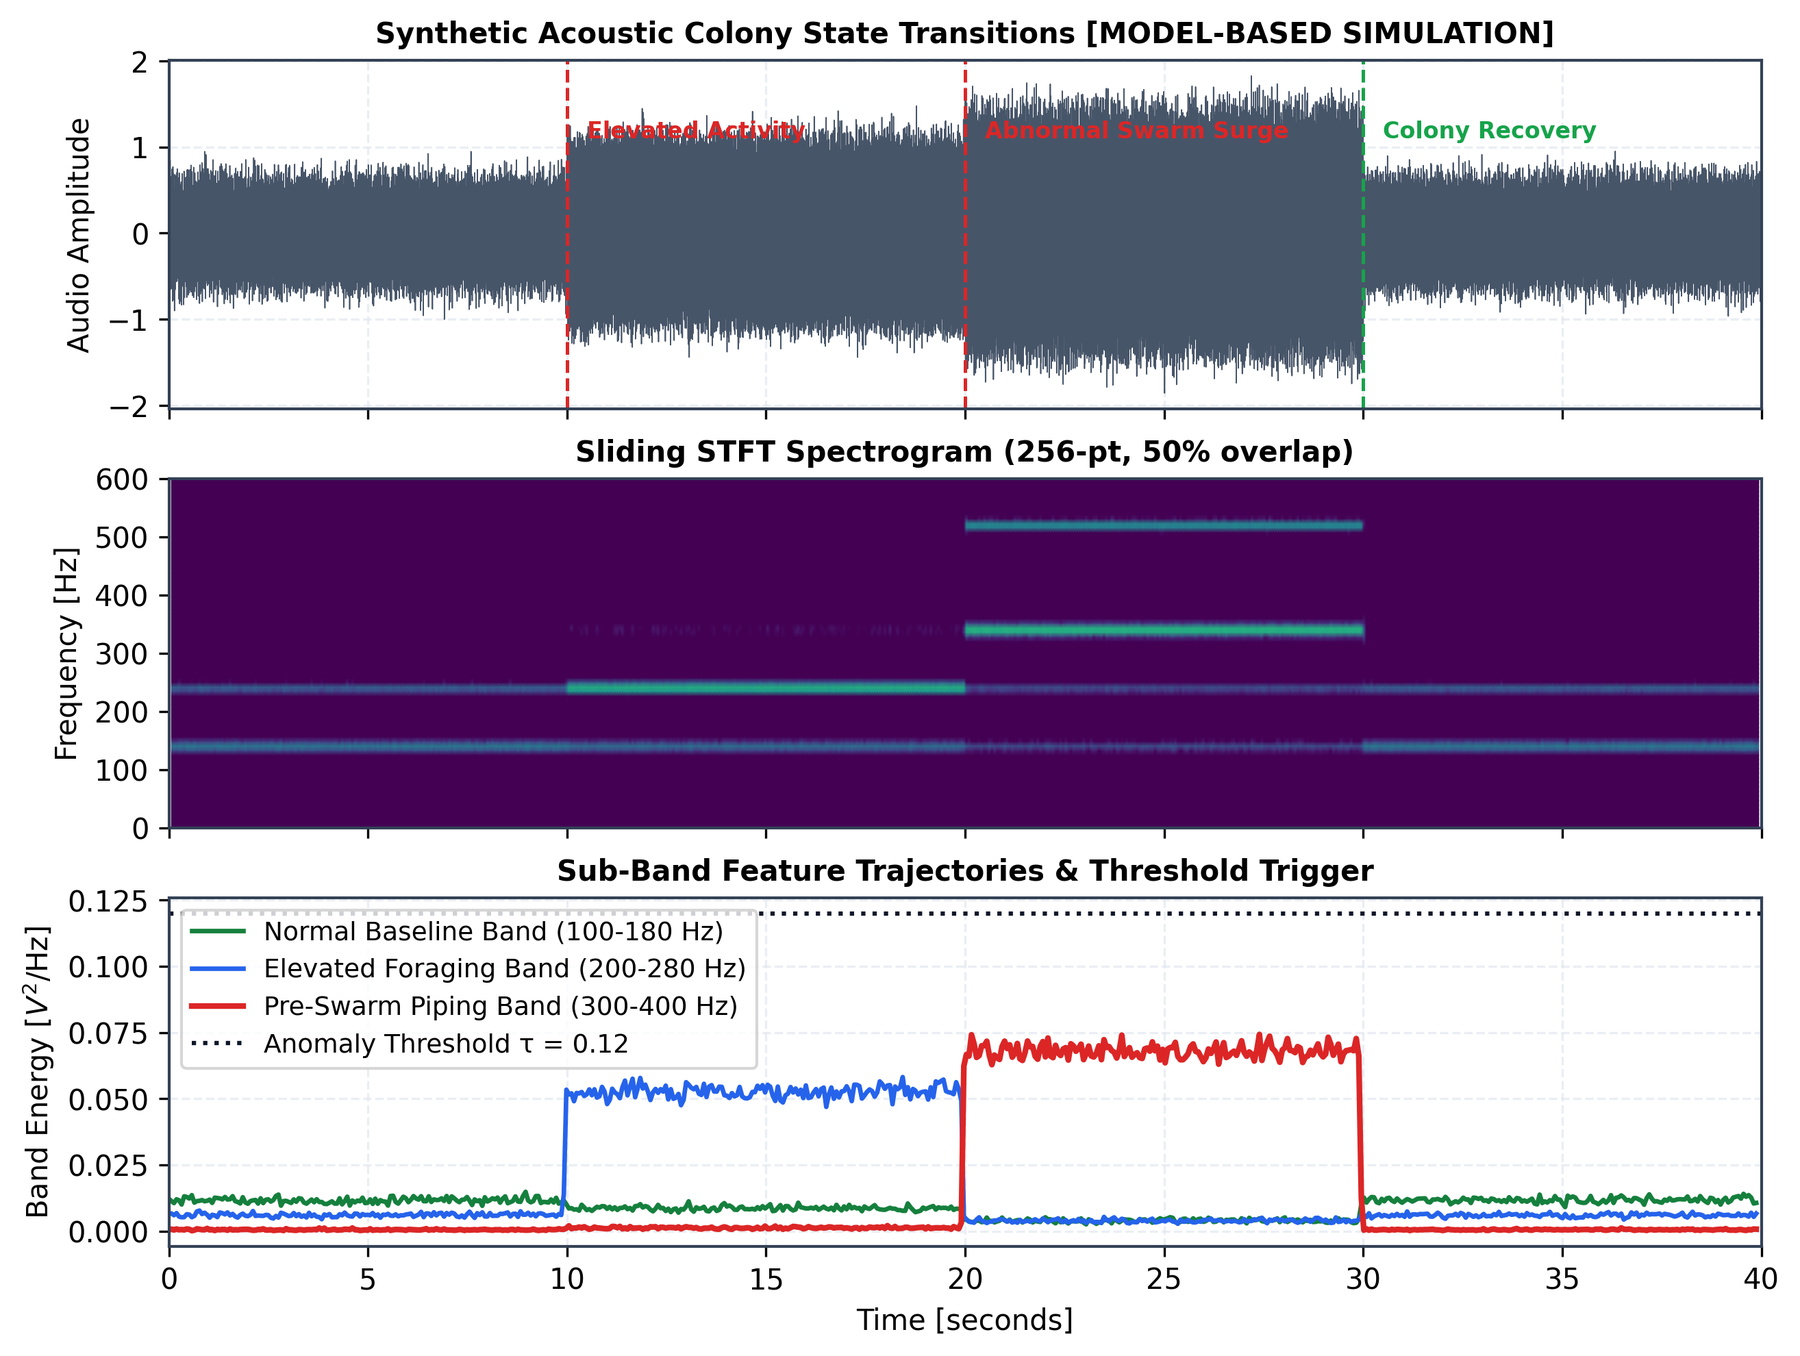
\includegraphics[width=0.27\textwidth]{figs/repo_acoustic_event_simulation.png}}
\caption{Model-based acoustic DSP illustrations generated by the repository's scripts (synthetic signals, $f_s = \SI{2}{kHz}$, 256-point Hann FFT, $\Delta f = \SI{7.81}{Hz}$) (\evA): (a) synthetic in-hive waveform; (b) spectrum with fanning and waggle peaks; (c) spectrogram with a pre-swarm component appearing at $t > \SI{5}{s}$; (d) sub-band energy trajectories; (e) rectangular versus Hann window resolving tones at 235 and \SI{255}{Hz}; (f) four-phase colony-state sequence with sub-band trajectories and an absolute threshold.}
\label{fig:dsp}
\end{figure*}

\begin{table}[!t]
\caption{Acoustic Front-End Design Space (Bins per Band)}
\label{tab:dsp}
\centering
\footnotesize
\setlength{\tabcolsep}{3.5pt}
\resizebox{\columnwidth}{!}{%
\begin{tabular}{@{}rrrrrrc@{}}
\toprule
$f_s$ (Hz) & $N$ & $\Delta f$ (Hz) & $f_\mathrm{Nyq}$ (Hz) & Frame (ms) & Buffer (kB) & $b_1/b_2/b_3/b_4$\\
\midrule
2000  & 256  & 7.81  & 1000 & 128 & 2.0  & 11/26/39/alias.\\
16000 & 256  & 62.50 & 8000 & 16  & 2.0  & 1/3/5/7\\
16000 & 2048 & 7.81  & 8000 & 128 & 16.0 & 11/26/39/51\\
8000  & 1024 & 7.81  & 4000 & 128 & 8.0  & 11/26/39/51\\
\textbf{4000} & \textbf{512} & \textbf{7.81} & \textbf{2000} & \textbf{128} & \textbf{4.0} & \textbf{11/26/39/51}\\
\bottomrule
\end{tabular}}
\\[2pt]\parbox{\columnwidth}{\footnotesize Bands $b_1$--$b_4$: \SIrange{100}{180}{Hz}, \SIrange{200}{400}{Hz}, \SIrange{450}{750}{Hz}, \SIrange{800}{1200}{Hz}. Bold: recommended (\SI{16}{kHz} I$^2$S decimated by 4). Buffer: two float frames.}
\end{table}

\begin{figure*}[!t]
\centering
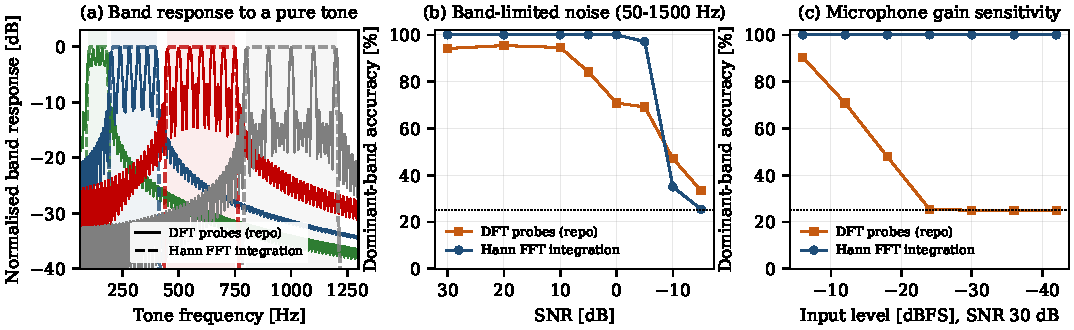
\includegraphics[width=\textwidth]{figs/fig_acoustic.pdf}
\caption{Acoustic robustness audit (\evA). (a) Normalised band response to a pure tone for the repository's DFT-probe estimator (solid) and Hann-windowed FFT integration (dashed); shading marks the four bands. (b) Dominant-band accuracy versus SNR with \SIrange{50}{1500}{Hz} noise. (c) Accuracy versus input level at \SI{30}{dB} SNR; the probe engine's absolute threshold drives it to chance level below \SI{-24}{dBFS}.}
\label{fig:acoustic}
\end{figure*}

\subsection{Gateway Advisory Classifier (\evT)}\label{sec:r-rf}
The Random Forest separates the four synthetic classes perfectly (five-fold accuracy and macro-F1 of 1.000, Fig.~\ref{fig:rf}(a)). This shows that the class-conditional distributions barely overlap, not that the model will generalise to field data. Under perturbations of one in-class standard deviation, macro-F1 drops to 0.975, and to 0.726 at three standard deviations (Fig.~\ref{fig:rf}(b)). The dominant acoustic frequency carries most of the decision (impurity importance 0.48, versus 0.20, 0.17 and 0.15 for mass, temperature and \COtwo{}). Losing the microphone reduces macro-F1 to 0.47 and losing \COtwo{} or the scale to 0.67 and 0.73, whereas losing brood temperature costs almost nothing (0.996; Fig.~\ref{fig:rf}(c)). The last result contradicts the biological prior that brood temperature is an early indicator of queen loss; it arises because the synthetic queenless class differs from healthy colonies mainly in its acoustic peak. Labelled field data are required before any accuracy figure can be claimed.

\begin{figure*}[!t]
\centering
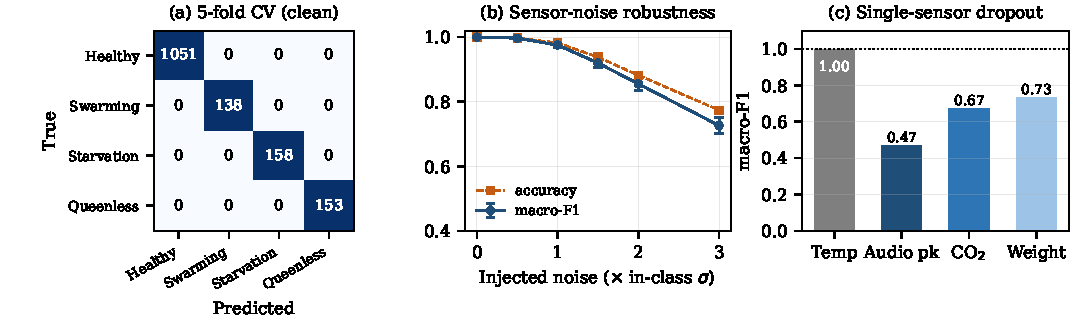
\includegraphics[width=\textwidth]{figs/fig_rf_eval.pdf}
\caption{Advisory Random Forest on the synthetic parametric dataset. (a) Five-fold cross-validated confusion matrix. (b) Accuracy and macro-F1 versus injected sensor noise in units of the healthy-class standard deviation (mean $\pm$ s.d.\ over 20 draws). (c) Macro-F1 when one sensor is replaced by its healthy-class median; the dotted line is the clean score.}
\label{fig:rf}
\end{figure*}

\subsection{Thermal Context and Multiphysics Models (\evA, \evS)}\label{sec:r-sim}
Fig.~\ref{fig:thermal} shows the repository's two-node lumped thermal model (brood heat capacity \SI{45}{kJ/K}, hive air \SI{85}{kJ/K}, $R_\mathrm{bh} = \SI{0.85}{K/W}$, $R_\mathrm{ha} = \SI{0.45}{K/W}$) with a proportional metabolic heater. Under a \SIrange{15}{35}{\celsius} diurnal ambient the brood stays within \SI{\pm1}{\celsius} of \SI{34.5}{\celsius} while the metabolic power varies between about 4.5 and \SI{12.5}{W}. Brood temperature alone therefore hides stress until compensation saturates, which motivates combining it with acoustic and \COtwo{} cues.

\begin{figure}[!t]
\centering
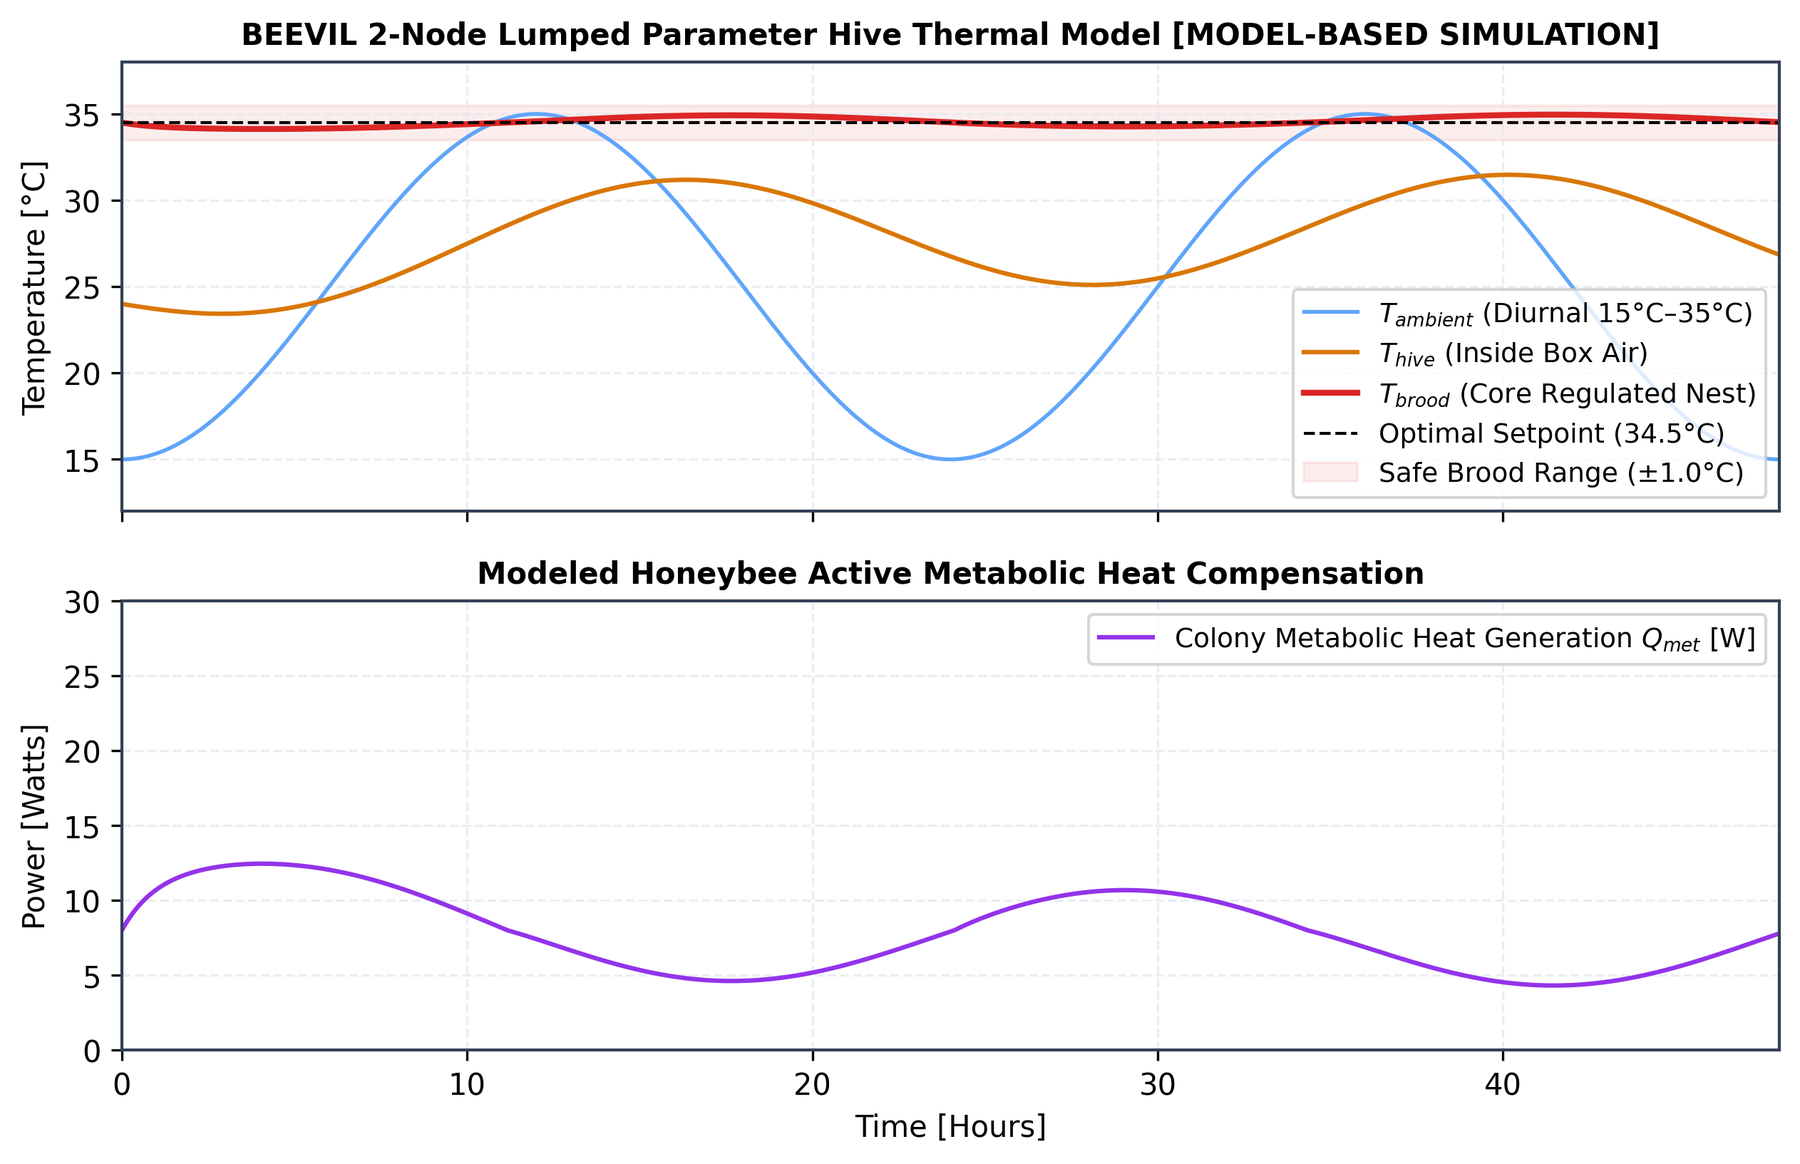
\includegraphics[width=\columnwidth]{figs/repo_hive_thermal_model.png}
\caption{Two-node lumped hive thermal model from the repository (\evA): ambient, hive-air and regulated brood temperatures (top) and the metabolic heat the colony must supply (bottom) over \SI{48}{h}.}
\label{fig:thermal}
\end{figure}

Table~\ref{tab:ansys} and Fig.~\ref{fig:ansys} summarise the solved ANSYS models. The transient thermal model of the hive with brood cluster, cell and electronics (85\,109 nodes) was cooled from \SI{22}{\celsius} by convection (\SI{12}{W.m^{-2}.K^{-1}}) to an ambient falling from \SI{15}{\celsius} to \SI{-15}{\celsius} over \SI{3}{h}. After \SI{4}{h} the exterior reached \SI{-14.7}{\celsius} while the warmest interior node was still at \SI{22.0}{\celsius}, so the interior time constant greatly exceeds the \SI{4}{h} horizon. With metabolic heat disabled this is a passive worst case; a \SI{24}{h} run with the cluster as a heat source is the next step. A \SI{2}{m} steel gateway mast under a lateral load deflected \SI{34.1}{mm} at the panel with a peak von Mises stress of \SI{109.8}{MPa} at the base, a safety factor of 2.3 against a \SI{250}{MPa} yield strength. The load magnitude was not stored with the result and must be restated before this factor can be tied to a wind speed. A modal analysis of the enclosure placed its first six modes between 36.2 and \SI{41.2}{kHz}, and a static load deflected it by \SI{31}{nm}; both reflect a solid-body approximation, and a shell model with the PCB and cell is needed to test acoustic coupling into the \SIrange{100}{1200}{Hz} band. The HFSS model of the \SI{865}{MHz} antenna in the hive converged, but $|S_{11}| \approx \SI{-1e-5}{dB}$ across \SIrange{0.7}{1.0}{GHz} and the solver warns that only one conductor touches the lumped port. The excitation therefore has no return path and the model does not yet describe a radiating antenna, so its \SI{-6.5}{dB} peak gain should not be used; the link budget above relies on catalogue antenna gains instead. The SPEOS solar-irradiance model is set up but not yet solved.

\begin{table*}[!t]
\caption{ANSYS Models With Documented Solutions (\evS)}
\label{tab:ansys}
\centering
\footnotesize
\begin{tabular}{@{}>{\raggedright\arraybackslash}p{2.2cm}>{\raggedright\arraybackslash}p{2.6cm}>{\raggedright\arraybackslash}p{4.4cm}>{\raggedright\arraybackslash}p{3.9cm}>{\raggedright\arraybackslash}p{3.25cm}@{}}
\toprule
Model & Solver & Domain and boundary conditions & Key output & Status / evidence\\
\midrule
Hive-node transient thermal & Mechanical/MAPDL 2026 R1, quasi-linear transient & 3 solids + surface; 85\,109 nodes, 49\,435 elements; pine, brood cluster, LiPo, FR-4, ABS; $T_0 = \SI{22}{\celsius}$; $h = \SI{12}{W.m^{-2}.K^{-1}}$; ambient 15 $\rightarrow$ \SI{-15}{\celsius} in \SI{5}{\celsius} steps every \SI{30}{min}; no internal heat & At \SI{4}{h}: $T_\mathrm{min} = \SI{-14.73}{\celsius}$ (exterior), $T_\mathrm{max} = \SI{22.0}{\celsius}$ & Solved; 243 substeps, \SI{240}{s} wall time (solver log)\\
Gateway mast & Mechanical static structural & $\approx\SI{2}{m}$ steel mast with top plate; fixed base; lateral force (magnitude not recorded) & $\delta_\mathrm{max} = \SI{34.1}{mm}$; $\sigma_\mathrm{vM,max} = \SI{109.8}{MPa}$; SF $\approx 2.3$ & Solved (screenshot)\\
Enclosure modal & Mechanical modal & $\approx\SI{0.1}{m}$ solid enclosure body; fixed support & $f_{1\ldots6}$ = 36.18, 36.93, 36.97, 40.03, 40.27, \SI{41.17}{kHz} & Solved (screenshot)\\
Enclosure static & Mechanical static structural & same body; applied force (magnitude not recorded) & $\delta_\mathrm{max} = \SI{31.4}{nm}$ & Solved (screenshot)\\
Solar irradiance & SPEOS 2026 R1 & panel plate, irradiance sensor, direct simulation & --- & Set up, not solved\\
Antenna in hive & HFSS 2025 R2.4, driven modal & FR-4 and honey materials; \SIrange{0.70}{1.00}{GHz} interpolating sweep (100 points, converged) & $|S_{11}| \approx \SI{-1e-5}{dB}$; peak gain \SI{-6.5}{dB}; port warning & Invalid excitation; to be fixed\\
\bottomrule
\end{tabular}
\end{table*}

\begin{figure*}[!t]
\centering
\subfloat[]{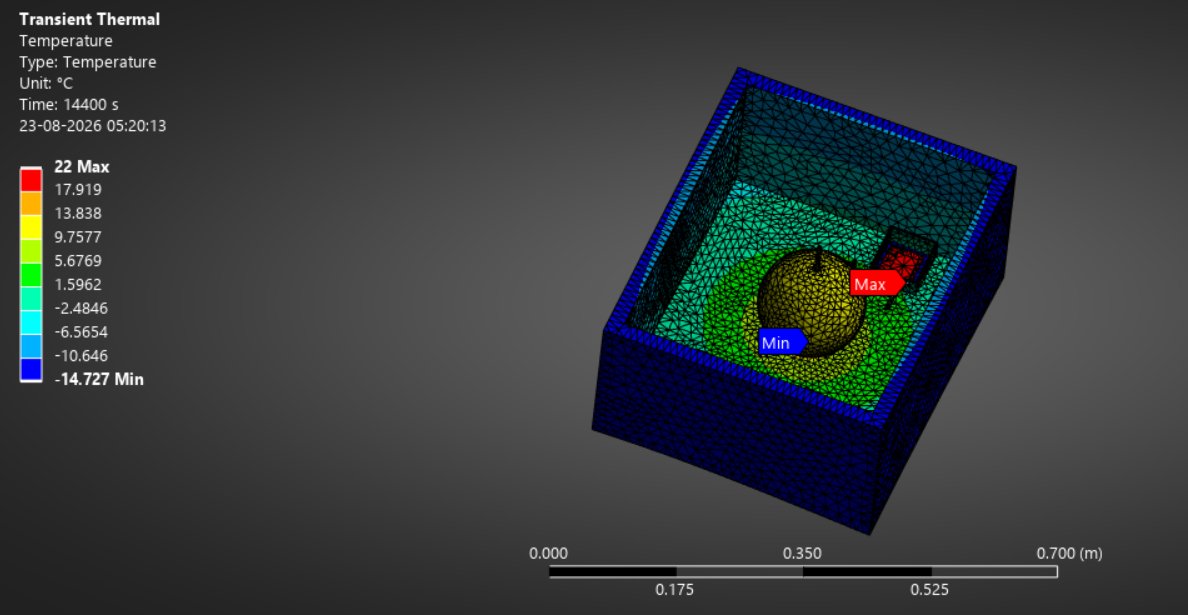
\includegraphics[width=0.245\textwidth]{figs/ansys_thermal.png}}\hfil
\subfloat[]{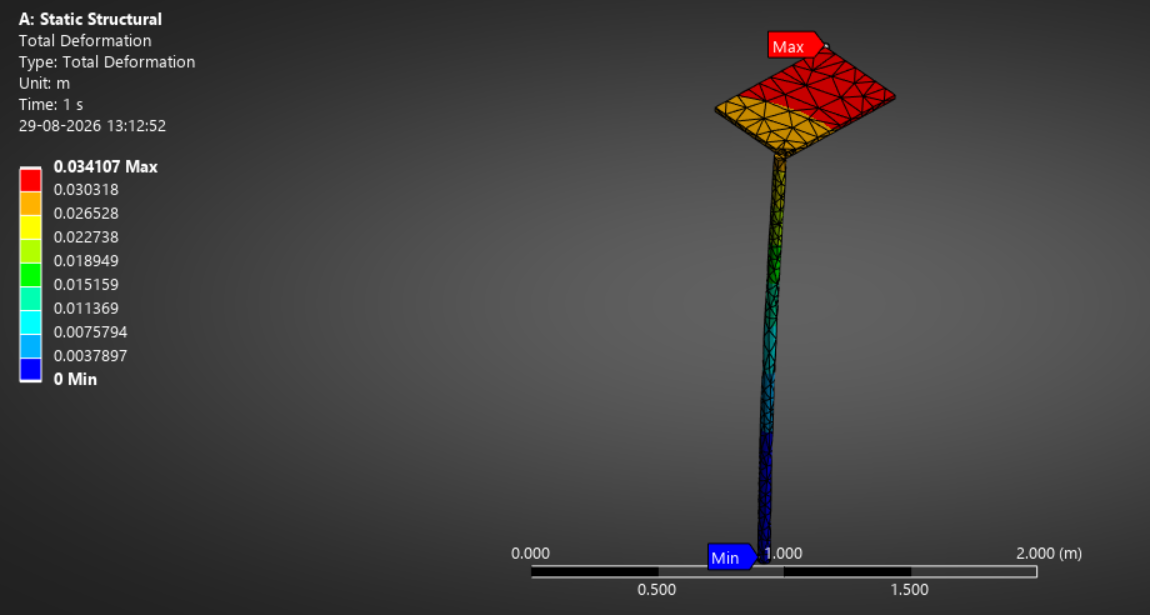
\includegraphics[width=0.245\textwidth]{figs/ansys_mast_def.png}}\hfil
\subfloat[]{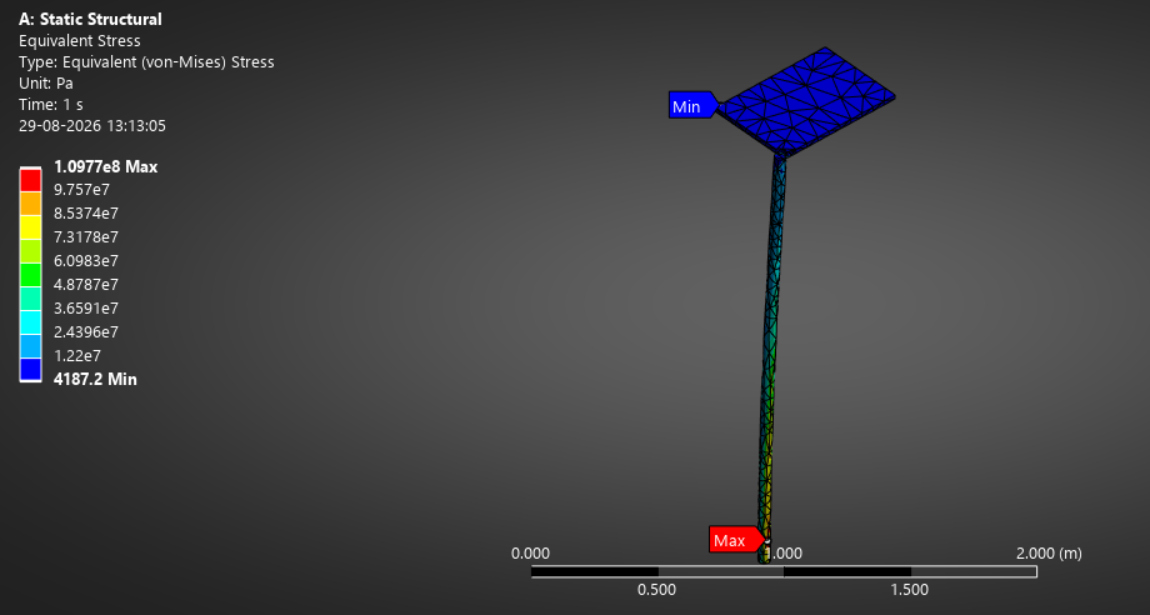
\includegraphics[width=0.245\textwidth]{figs/ansys_mast_vm.png}}\hfil
\subfloat[]{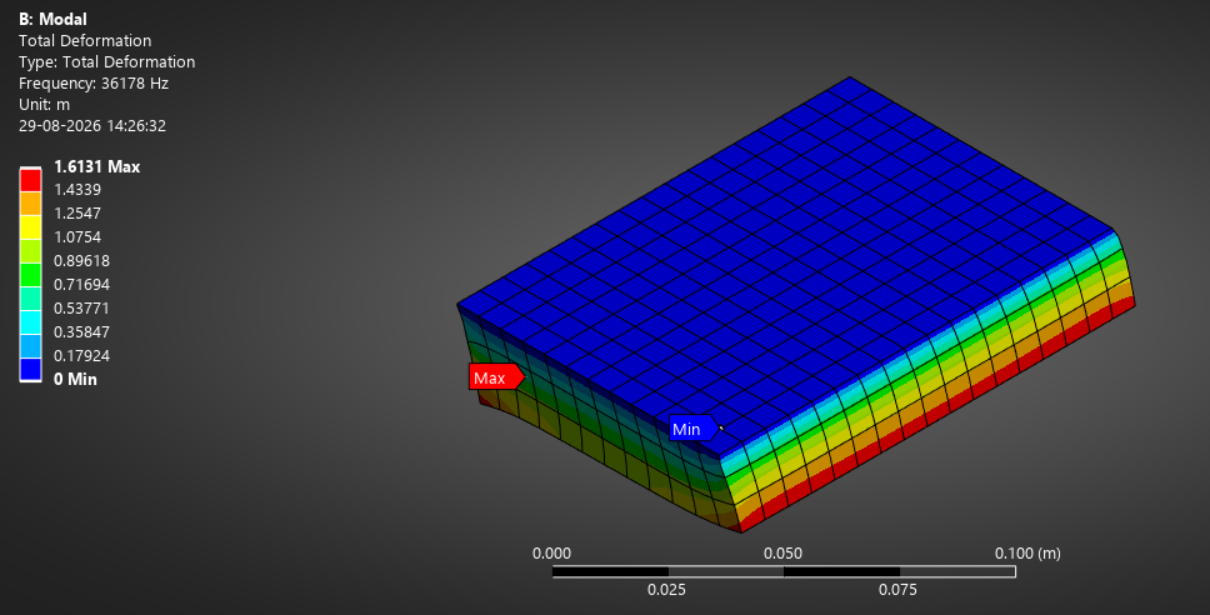
\includegraphics[width=0.245\textwidth]{figs/ansys_modal.png}}\\[-1pt]
\subfloat[]{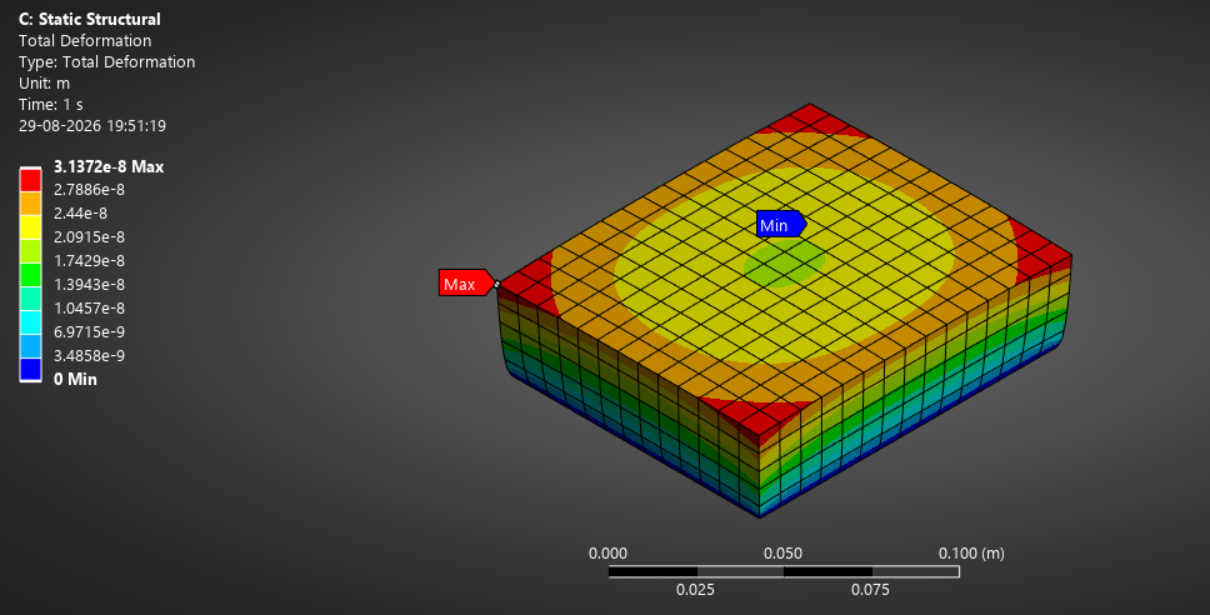
\includegraphics[width=0.245\textwidth]{figs/ansys_encl.png}}\hfil
\subfloat[]{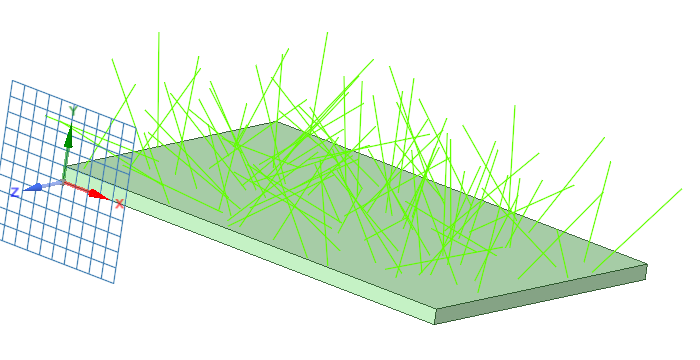
\includegraphics[width=0.245\textwidth]{figs/ansys_speos.png}}\hfil
\subfloat[]{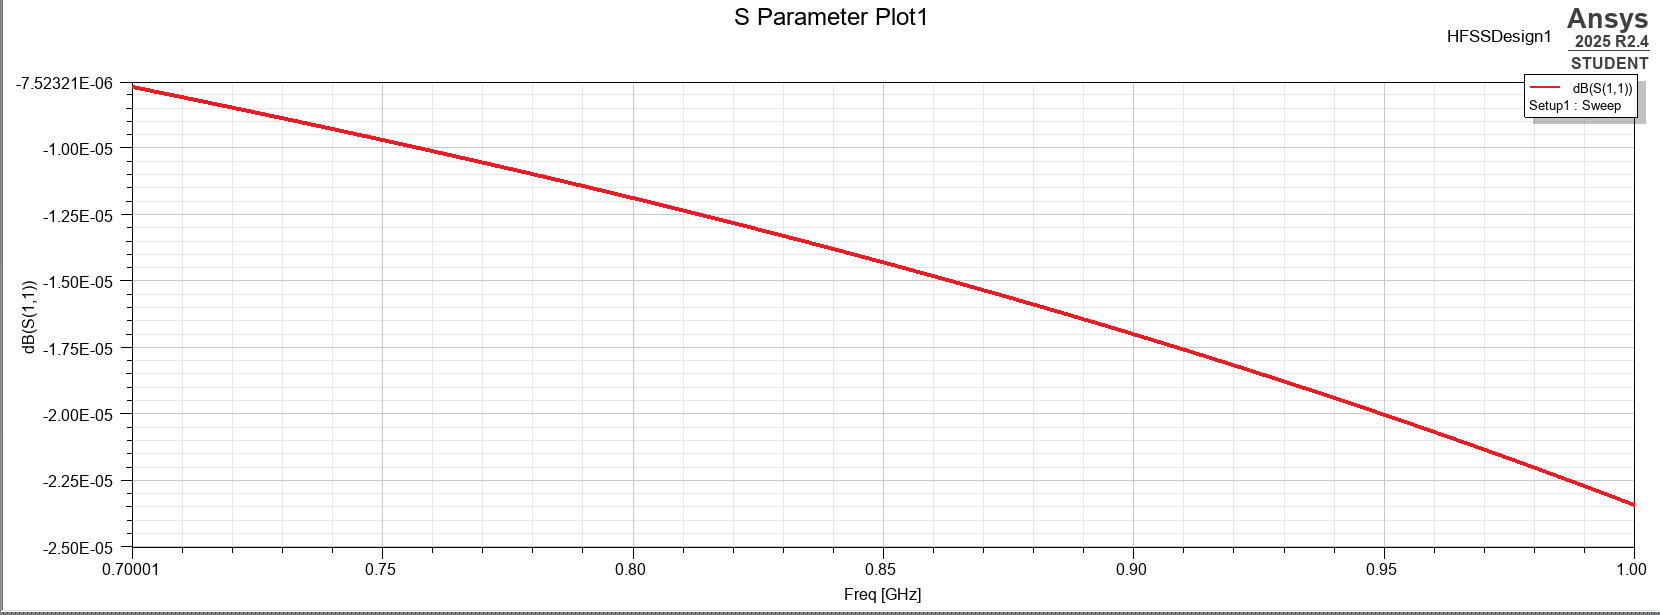
\includegraphics[width=0.245\textwidth]{figs/ansys_s11.png}}\hfil
\subfloat[]{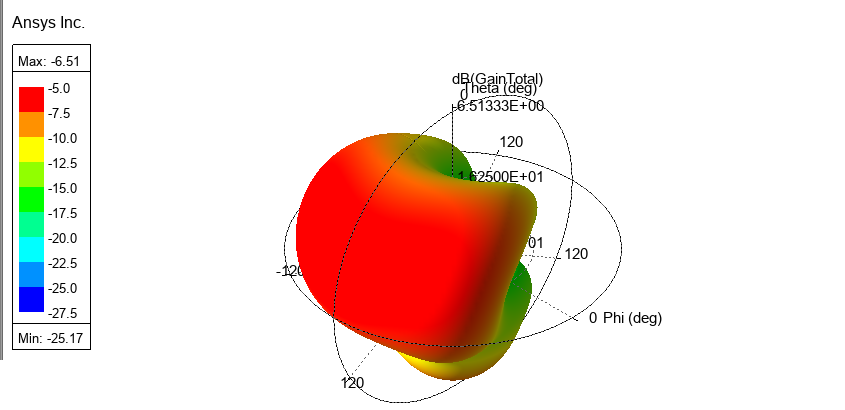
\includegraphics[width=0.21\textwidth]{figs/ansys_gain.png}}
\caption{ANSYS solver screenshots from the project repository (\evS): (a) hive-node temperature after \SI{4}{h} of passive cooling; (b) total deformation and (c) von Mises stress of the gateway mast; (d) first enclosure mode (\SI{36.18}{kHz}); (e) static deformation of the enclosure; (f) SPEOS solar set-up; (g) HFSS $|S_{11}|$ (scale $10^{-5}$ dB) revealing the invalid port; (h) corresponding 3-D gain pattern.}
\label{fig:ansys}
\end{figure*}

% ===========================================================================
\section{Discussion}\label{sec:disc}
% ===========================================================================
\subsection{What the Evidence Supports}
The architecture, telemetry contract and gateway software are implemented and reproducibly tested, and the node firmware compiles and exercises its on-chip measurements. Radio, energy, detection and acoustic performance are supported by analysis with stated assumptions. The field node has not yet transmitted hive data over the air, and we make no claim of field accuracy. Several figures in earlier project documents (including a 15 km range, 94% to 97% diagnostic accuracies, multi-year autonomy, and antenna matching of -25 dB) are not supported by the executable artefacts and are superseded by the analysis above.

\subsection{Design Changes Motivated by This Study}
\begin{enumerate}
\item Add a flags byte and a sequence number to the frame (35 bytes, \SI{77.1}{ms} at SF7).
\item Use time-slotted or multi-channel access beyond about 20 hives per channel, and raise the gateway antenna before raising SF.
\item Measure \COtwo{} every \SI{30}{min} with the SCD41 power-gated.
\item Replace the firmware detector by Page's CUSUM with a physiological target and $k \approx \SI{0.25}{\celsius}$, $h \approx 8$, recalibrated on field data.
\item Implement band energies by FFT integration on a decimated \SI{4}{kHz} stream, decide on relative energies, and gate on calibrated loudness.
\item Drive the gateway HAT through its UART interface (the ``T'' in E22-900T22S denotes a UART module) with air parameters matched to the node, and complete the SX1262 transmit path on the node.
\item Fix the HFSS port, model the enclosure as a shell with PCB and cell, and run a \SI{24}{h} thermal case with metabolic heat.
\end{enumerate}

\subsection{Limitations and Threats to Validity}
The classifier is trained and tested on synthetic data, and the acoustic study uses synthetic tones; the Zenodo real-audio benchmarks were not re-executed. Energy figures use datasheet typical values and an assumed board sleep floor. The radio results rest on a flat-ground two-ray model, an empirical foliage model, an assumed hive-body loss and pure ALOHA without capture. The CUSUM study assumes Gaussian AR(1) variability with $\sigma = \SI{0.15}{\celsius}$, which must be verified in real brood nests. The ingestion benchmark ran on an x86 host, not on the Raspberry Pi. Finally, the project documentation contains inconsistent values for several parameters (FFT size and sampling rate, cell capacity, airtime); throughout this paper we used the values in executable code and in manufacturer datasheets.

\subsection{Planned Field Validation}
A five-hive pilot with \textit{Apis mellifera} and \textit{Apis cerana indica} colonies will (i) measure sleep and active current with a power profiler; (ii) measure RSSI and delivery versus distance and gateway antenna height; (iii) collect labelled audio to calibrate band edges and the loudness gate for both species; (iv) estimate $\sigma$ and $\rho$ of brood temperature to set the CUSUM parameters; and (v) evaluate the advisory model on field labels.

% ===========================================================================
\section{Conclusion}\label{sec:concl}
% ===========================================================================
Beevil Knievel shows that a complete, open hive-monitoring pipeline, integrating in-comb multimodal sensing, on-node feature extraction, a 33-byte LoRa frame, and an offline, power-loss-hardened gateway, can be specified and verified in software before field deployment, and that doing so exposes design issues early. Our analyses indicate that a 100-hive yard can be served at SF7 with scheduled or multi-channel access over \SIrange{0.6}{1.3}{km}, that \COtwo{} sensing rather than radio dominates node energy, that brood-cooling detection must account for autocorrelated variability, and that relative, FFT-integrated band energies are needed for gain-robust acoustic decisions. The next step is the field pilot, which will replace the modelled assumptions with measurements.

\section*{Data Availability}
Source code, firmware, simulation files and the scripts that regenerate every figure and table in Section~\ref{sec:results} are available in the project repository (\url{https://github.com/atharveeee-netizen/beevil-knievel})~\cite{beevilrepo}.

\section*{Acknowledgment}
The authors thank the IEEE Humanitarian Activities Committee (HAC) and Special Interest Group on Humanitarian Technology (SIGHT) team for project support, and L.~Shankar for contributions to the Beevil Knievel prototype design.

\bibliographystyle{IEEEtran}
\bibliography{references}

\end{document}
